\subsection{UNIVERSAL PROBLEM FOR DERIVATIONS; COMMUTATIVE CASE}

Suppose now that A is a commutative K-algebra and E an A-module; E can be considered as an (A, A)-bimodule whose two external laws are identical with the given A-module law. On the other hand the (A, A)-bimodule structure on \(A \otimes_{K} A\) is identical with its \((A \otimes_{K} A)\) -module structure arising from the commutative ring structure on \(A \otimes_{K} A\) , since in this case, for x, y, u, v in A,

\[
x. (u \otimes v). y = (x u) \otimes (v y) = (x u) \otimes (y v) = (x \otimes y) (u \otimes v).
\]

The kernel \(\mathfrak{J}\) of \(m\) is therefore in this case an ideal of the ring \(\mathbf{A} \otimes_{\mathbb{K}} \mathbf{A}\) and, as \(m: \mathbf{A} \otimes_{\mathbb{K}} \mathbf{A} \to \mathbf{A}\) is surjective, \((\mathbf{A} \otimes_{\mathbb{K}} \mathbf{A}) / \mathfrak{J}\) is isomorphic to \(\mathbf{A}\) ; if also \(\mathbf{E}\) is considered as an \((\mathbf{A} \otimes_{\mathbb{K}} \mathbf{A})\) -module by means of \(m\) (in other words the \((\mathbf{A} \otimes_{\mathbb{K}} \mathbf{A})\) -module \(m_*(\mathbf{E})\) ), the \((\mathbf{A}, \mathbf{A})\) -bimodule homomorphisms \(\mathfrak{J} \to \mathbf{E}\) are identified with the \((\mathbf{A} \otimes_{\mathbb{K}} \mathbf{A})\) -module homomorphisms \(\mathfrak{J} \to \mathbf{E}\) ( \(\S 4, no. 3\) ), in other words there is a canonical \(\mathbf{K}\) -module isomorphism.

\[
\operatorname{Hom} _ {(\mathbf {A}, \mathbf {A})} (\mathfrak{J} , \mathrm{E}) \rightarrow \operatorname{Hom} _ {\mathbf {A} \otimes_ {\mathbf {K}} \mathbf {A}} (\mathfrak{J} , \mathrm{E}).
\]

On the other hand, \(\mathfrak{J}\mathbf{E} = \{0\}\) , for the elements \(1 \otimes x - x \otimes 1\) generate \(\mathfrak{J}\) as an \((\mathbf{A} \otimes_{\mathbb{K}} \mathbf{A})\) -module (no. 10, Lemma 1) and, for all \(z \in \mathbf{E}\) ,

\[
(1 \otimes x - x \otimes 1) z = 0
\]

by virtue of the definition of the \((\mathbf{A} \otimes_{\mathbf{K}} \mathbf{A})\) -module structure on E. Since \(\mathfrak{J}\) is contained in the annihilator of the \((\mathbf{A} \otimes_{\mathbf{K}} \mathbf{A})\) -module E and the \(((\mathbf{A} \otimes_{\mathbf{K}} \mathbf{A})/\mathfrak{J})\) -module structure on E is by definition just the initial A-module structure given on E, there is, taking account of the canonical isomorphism of

\[
\mathfrak{J} \otimes_ {\mathbf {K}} ((\mathbf {A} \otimes_ {\mathbf {K}} \mathbf {A}) / \mathfrak{J})
\]

onto \(\mathfrak{J} / \mathfrak{J}^2\) (§ 4, no. 1, Corollary 1 to Proposition 1), a canonical K-module isomorphism

\[
\operatorname{Hom} _ {\mathbf {A} \otimes_ {\mathbf {K}} \mathbf {A}} (\mathfrak{J} , \mathrm{E}) \rightarrow \operatorname{Hom} _ {\mathbf {A}} (\mathfrak{J} / \mathfrak{J}^ {2}, \mathrm{E}).
\]

Taking account of Proposition 17 of no. 10, it is seen that we have proved the following proposition:

PROPOSITION 18. Let A be a commutative K-algebra and \(\mathfrak{J}\) the ideal the kernel of the surjective canonical homomorphism \(m: \mathbf{A} \otimes_{\mathbf{K}} \mathbf{A} \to \mathbf{A}\) , so that A is isomorphic to \((\mathbf{A} \otimes_{\mathbf{K}} \mathbf{A}) / \mathfrak{J}\) and \(\mathfrak{J} / \mathfrak{J}^2\) has canonically an A-module structure. Let \(d_{\mathbf{A} / \mathbf{K}}: \mathbf{A} \to \mathfrak{J} / \mathfrak{J}^2\) be the K-linear mapping which associates with every \(x \in \mathbf{A}\) the class of \(x \otimes 1 - 1 \otimes x\) modulo \(\mathfrak{J}^2\) . The mapping \(d_{\mathbf{A} / \mathbf{K}}\) is a K-derivation and, for every A-module E and every K-derivation D: \(\mathbf{A} \to \mathbf{E}\) , there exists one and only one A-linear mapping \(g: \mathfrak{J} / \mathfrak{J}^2 \to \mathbf{E}\) such that \(\mathrm{D} = g \circ d_{\mathbf{A} / \mathbf{K}}\) .

The A-module \(\mathfrak{J} / \mathfrak{J}^2\) is called the A-module of K-differentials of A and is denoted by \(\Omega_{\mathbf{K}}(\mathbf{A})\) ; for all \(x \in \mathbf{A}\) , \(d_{\mathbf{A} / \mathbf{K}}(x)\) (also denoted by \(dx\) ) is called the differential of \(x\) ; it has been seen (no. 10, lemma 1) that the elements \(d_{\mathbf{A} / \mathbf{K}}(x)\) , for \(x \in \mathbf{A}\) , form a generating system of the A-module \(\Omega_{\mathbf{K}}(\mathbf{A})\) . Proposition 18 shows that the mapping \(g \mapsto g \circ d_{\mathbf{A} / \mathbf{K}}\) is a canonical A-module isomorphism

\[
\phi_ {\mathbf {A}}: \operatorname{Hom} _ {\mathbf {A}} (\Omega_ {\mathbf {K}} (\mathbf {A}), \mathrm{E}) \rightarrow \mathrm{D} _ {\mathbf {K}} (\mathrm{A}, \mathrm{E})
\]

(the A-module structure on \(D_{K}(A, E)\) being defined by Proposition 7 of no. 5).

The ordered pair \((\Omega_{\mathbf{K}}(\mathbf{A}), d_{\mathbf{A}/\mathbf{K}})\) is therefore the solution of the universal mapping problem where \(\Sigma\) is the species of A-module structure and the \(\alpha\) -mappings the K-derivations from A to an A-module (Set Theory, IV, §3, no. 1).

Example. Let M be a K-module; it follows from Proposition 14 of no. 9 that for every S(M)-module E, the mapping D ↦ D \textbar{} M defines an S(M)-module isomorphism of D\_K(S(M), E) onto Hom\_K(M, E); on the other hand, since E is an S(M)-module, Hom\_K(M, E) is canonically isomorphic to

\[
\operatorname{Hom} _ {\mathbf {S} (\mathbf {M})} (\mathbf {M} \otimes_ {\mathbf {K}} \mathbf {S} (\mathbf {M}), \mathbf {E}),
\]

every K-homomorphism of M into E being uniquely expressible in the form \(x \mapsto h(x \otimes 1)\) , where

\[
h \in \operatorname{Hom} _ {\mathbf {S} (\mathbf {M})} (\mathbf {M} \otimes_ {\mathbf {K}} \mathbf {S} (\mathbf {M}), \mathbf {E})
\]

(II, § 5, no. 1). Let \(\mathbf{D}_0\) be the K-derivation \(\mathbb{S}(\mathbf{M}) \to \mathbf{M} \otimes_{\mathbb{K}} \mathbb{S}(\mathbf{M})\) whose restriction to \(\mathbf{M}\) is the canonical homomorphism \(x \mapsto x \otimes 1\) ; every K-derivation \(\mathbf{D}: \mathbb{S}(\mathbf{M}) \to \mathbf{E}\) can therefore be written uniquely as \(h \circ \mathbf{D}_0\) with

\[
h \in \operatorname{Hom} _ {\mathbf {S} (\mathbf {M})} (\mathbf {M} \otimes_ {\mathbf {K}} \mathbf {S} (\mathbf {M}), \mathbf {E}).
\]

By the uniqueness of a solution of a universal mapping problem, it is seen that there exists a unique S(M)-module isomorphism

\[
\omega : \mathbf {M} \otimes_ {\mathbf {K}} \mathbf {S} (\mathbf {M}) \rightarrow \Omega_ {\mathbf {K}} (\mathbf {S} (\mathbf {M}))
\]

such that \(\mathbf{D}_0\circ \omega = d_{\mathbb{S}(\mathbf{M}) / \mathbb{K}}\) ; in other words, for all \(x\in \mathbf{M}\) \(\omega (x\otimes 1) = dx.\) In particular, if \(\mathbf{M}\) is a free K-module with basis \((e_{\lambda})_{\lambda \in \mathbf{L}},\Omega_{\mathbb{K}}(\mathbb{S}(\mathbf{M}))\) is a free S(M)-module with basis the set of differentials \(de_{\lambda}\) . Consider in particular the case where \(\mathrm{L} = [1,n]\) , so that \(\mathbb{S}(\mathbf{M})\) is identified with the polynomial algebra \(\mathbf{K}[\mathbf{X}_1,\dots ,\mathbf{X}_n]\) (§ 6, no. 6); for every polynomial \(\mathrm{P}\in \mathrm{K}[\mathrm{X}_1,\dots ,\mathrm{X}_n]\) , we can write uniquely

\[
d \mathrm{P} = \sum_ {i = 1} ^ {n} \mathrm{D} _ {i} \mathrm{P}. d \mathrm{X} _ {i}
\]

with \(D_{i}P \in K[X_{1}, \ldots, X_{n}]\) and, by virtue of the above, the mappings \(P \mapsto D_{i}P\) are the K-derivations of \(K[X_{1}, \ldots, X_{n}]\) corresponding to the coordinate forms on \(\Omega_{K}(S(M))\) for the basis \((dX_{i})\) ; we also write \(\frac{\partial P}{\partial X_{i}}\) instead of \(D_{i}P\) and this is called the partial derivative of P with respect to \(X_{i}\) .

\subsection{FUNCTORIAL PROPERTIES OF K-DIFFERENTIALS}

PROPOSITION 19. Let

\[
\begin{array}{c c c} \mathrm{K} & \xrightarrow {\rho} & \mathrm{K} ^ {\prime} \\ \Big \downarrow_ {\eta} & & \Big \downarrow_ {\eta^ {\prime}} \\ \mathrm{A} & \xrightarrow {u} & \mathrm{A} ^ {\prime} \end{array}
\]

be a commutative diagram of commutative ring homomorphisms, \(\eta\) (resp. \(\eta'\) ) making

A (resp. A') into a K-algebra (resp. K'-algebra). There exists one and only one A-linear mapping \(v: \Omega_{\mathbf{K}}(\mathbf{A}) \to \Omega_{\mathbf{K}'}(\mathbf{A}')\) rendering commutative the diagram

\pandocbounded{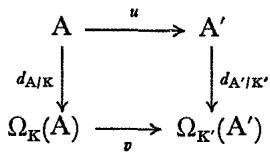
\includegraphics[keepaspectratio]{images/part004_9ff9737d.jpg}}

\(d_{\mathbf{A}^{\prime} / \mathbf{K}^{\prime}}\circ u\) is a K-derivation of A with values in the A-module \(\Omega_{\mathbf{K}^{\prime}}(\mathbf{A}^{\prime})\) ; the existence and uniqueness of \(v\) then follow from Proposition 18 of no. 11.

The mapping v of Proposition 19 will be denoted by \(\Omega(u)\) ; if there is a commutative diagram of commutative ring homomorphisms

\pandocbounded{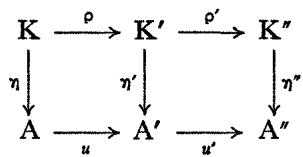
\includegraphics[keepaspectratio]{images/part004_26fbb1e8.jpg}}

it follows immediately from the uniqueness property of Proposition 19 that

\[
\Omega (u ^ {\prime} \circ u) = \Omega (u ^ {\prime}) \circ \Omega (u).
\]

Since \(\Omega_{\mathbf{K}'}(\mathbf{A}')\) is an \(\mathbf{A}'\) -module, from \(\Omega(u)\) we derive canonically an \(\mathbf{A}'\) -linear mapping

\[
\Omega_ {0} (u): \Omega_ {\mathbf {K}} (\mathrm{A}) \otimes_ {\mathrm{A}} \mathrm{A} ^ {\prime} \rightarrow \Omega_ {\mathbf {K} ^ {\prime}} (\mathrm{A} ^ {\prime})\tag{41}
\]

such that \(\Omega(u)\) is the composition of \(\Omega_0(u)\) and the canonical homomorphism \(i_{\mathbf{A}}: \Omega_{\mathbf{K}}(\mathbf{A}) \to \Omega_{\mathbf{K}}(\mathbf{A}) \otimes_{\mathbf{A}} \mathbf{A}'\) . For every \(\mathbf{A}'\) -module \(\mathbf{E}'\) , there is a commutative diagram

\pandocbounded{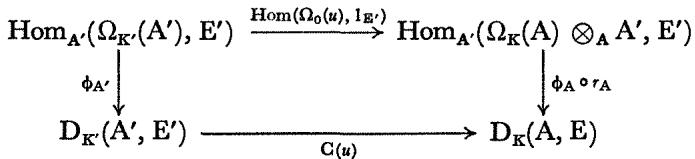
\includegraphics[keepaspectratio]{images/part004_95f64194.jpg}}

where \(\mathbf{C}(u)\) is the mapping \(D \mapsto D \circ u\) (no. 7, Proposition 9) and \(r_{A}\) is the canonical isomorphism

\[
\operatorname{Hom} \left(i _ {\mathrm{A}}, 1 _ {\mathrm{E} ^ {\prime}}\right): \operatorname{Hom} _ {\mathrm{A} ^ {\prime}} \left(\Omega_ {\mathrm{K}} (\mathrm{A}) \otimes_ {\mathrm{A}} \mathrm{A} ^ {\prime}, \mathrm{E} ^ {\prime}\right)\rightarrow \operatorname{Hom} _ {\mathrm{A}} \left(\Omega_ {\mathrm{K}} (\mathrm{A}), \mathrm{E} ^ {\prime}\right);
\]

this follows immediately from Proposition 19 and the definition of the isomorphisms \(\phi_{\mathbf{A}}\) and \(\phi_{\mathbf{A}^{\prime}}\) .

PROPOSITION 20. Suppose that \(\mathbf{A}' = \mathbf{A} \otimes_{\mathbb{K}} \mathbf{K}'\) , with \(\eta': \mathbf{K}' \to \mathbf{A}'\) and \(u: \mathbf{A} \to \mathbf{A}'\) the canonical homomorphisms. Then the \(\mathbf{A}'\) -linear mapping

\[
\Omega_ {0} (u): \Omega_ {\mathbf {K}} (\mathrm{A}) \otimes_ {\mathbf {A}} \mathrm{A} ^ {\prime} \rightarrow \Omega_ {\mathbf {K} ^ {\prime}} (\mathrm{A} ^ {\prime})
\]

is an isomorphism.

By virtue of the fact that in diagram (42) the vertical arrows are bijective, it reduces to proving that, for every A'-module E', the homomorphism C(u):D → D ∘ u in diagram (42) is bijective (II, § 2, no. 1, Theorem 1). Now Hom(u, 1\_E') : Hom\_K'(A ⊗\_K K', E') → Hom\_K(A, E') is an isomorphism (II, § 5, no. 1, Proposition 1) and C(u) is its restriction to D\_K'(A', E') and hence is injective; moreover, if f: A' → E' is a K'-linear mapping such that

\[
f \circ u: \mathrm{A} \rightarrow \mathrm{E} ^ {\prime}
\]

is a K-derivation, it follows immediately from the fact that \(f\) is \(\mathbf{K}'\) -linear and the fact that \(f((x \otimes 1)(y \otimes 1)) = (y \otimes 1)f(x \otimes 1) + (x \otimes 1)f(y \otimes 1)\) for \(x, y\) in A, that \(f\) is a \(\mathbf{K}'\) -derivation, the elements \(x \otimes 1\) for \(x \in A\) forming a generating system of the \(\mathbf{K}'\) -module \(A'\) ; this completes the proof that \(C(u)\) is bijective.

From now on we confine our attention to the case where \(\rho: \mathbf{K} \to \mathbf{K}'\) is the identity mapping of \(\mathbf{K}\) ; every K-algebra homomorphism \(u: \mathbf{A} \to \mathbf{B}\) is therefore mapped to a B-linear mapping

\[
\Omega_ {0} (u): \Omega_ {\mathbf {K}} (\mathrm{A}) \otimes_ {\mathbf {K}} \mathrm{B} \rightarrow \Omega_ {\mathbf {K}} (\mathrm{B}).\tag{43}
\]

On the other hand, we can consider the B-module of A-differentials \(\Omega_{\mathbf{A}}(\mathbf{B})\) since B is an A-algebra by means of u; the canonical derivation \(d_{\mathrm{B/A}}: \mathbf{B} \to \Omega_{\mathbf{A}}(\mathbf{B})\) being a fortiori a K-derivation, it factorizes uniquely into

\[
\mathbf {B} \xrightarrow {d _ {\mathbf {B} / \mathbf {K}}} \Omega_ {\mathbf {K}} (\mathbf {B}) \xrightarrow {\Omega_ {u}} \Omega_ {\mathbf {A}} (\mathbf {B})
\]

where \(\Omega_{u}\) is a B-linear mapping (no. 11, Proposition 18). For every B-module E, there is a commutative diagram

\[
\begin{array}{c} \operatorname{Hom} _ {\mathbf {B}} (\Omega_ {\mathbf {A}} (\mathbf {B}), \mathrm{E}) \xrightarrow {\operatorname{Hom} (\Omega_ {u} , 1 _ {\mathbf {E}})} \operatorname{Hom} _ {\mathbf {B}} (\Omega_ {\mathbf {K}} (\mathbf {B}), \mathrm{E}) \\ \phi_ {\mathbf {A}, \mathbf {B}} \Biggl \downarrow \\ \mathrm{D} _ {\mathbf {A}} (\mathrm{B}, \mathrm{E}) \xrightarrow [ j _ {u} ]{} \mathrm{D} _ {\mathbf {K}} (\mathrm{B}, \mathrm{E}) \end{array}\tag{44}
\]

where \(j_{u}\) is the canonical injection (no. 7); this follows immediately from Proposition 18 of no. 11.

PROPOSITION 21. The sequence of B-linear mappings

\[
\Omega_ {\mathbf {K}} (\mathrm{A}) \otimes_ {\mathbf {A}} \mathrm{B} \xrightarrow {\Omega_ {0} (u)} \Omega_ {\mathbf {K}} (\mathrm{B}) \xrightarrow {\Omega_ {u}} \Omega_ {\mathbf {A}} (\mathrm{B}) \to 0\tag{45}
\]

is exact.

It reduces to verifying that, for every B-module E, the sequence

\[
\begin{array}{c} 0 \to \operatorname{Hom} _ {\mathrm{B}} (\Omega_ {\mathrm{A}} (\mathrm{B}), \mathrm{E}) \xrightarrow {\operatorname{Hom} (\Omega_ {\mathrm{u}} , 1 _ {\mathrm{E}})} \operatorname{Hom} _ {\mathrm{B}} (\Omega_ {\mathrm{K}} (\mathrm{B}), \mathrm{E}) \\ \xrightarrow {\operatorname{Hom} (\Omega_ {0} (u) , 1 _ {\mathrm{E}})} \operatorname{Hom} _ {\mathrm{B}} (\Omega_ {\mathrm{K}} (\mathrm{A}) \otimes_ {\mathrm{A}} \mathrm{B}, \mathrm{E}) \end{array}
\]

is exact (II, §2, no. 1, Theorem 1); but by virtue of the fact that in the commutative diagrams (42) and (44) the vertical arrows are isomorphisms, it suffices to show that the sequence

\[
0 \longrightarrow \mathrm{D} _ {\mathrm{A}} (\mathrm{B}, \mathrm{E}) \xrightarrow {j _ {u}} \mathrm{D} _ {\mathrm{K}} (\mathrm{B}, \mathrm{E}) \xrightarrow {\mathrm{C} (u)} \mathrm{D} _ {\mathrm{K}} (\mathrm{A}, \mathrm{E})
\]

is exact, which is just Proposition 11 of no. 7.

We consider now the case where the K-algebra homomorphism \(u: \mathbf{A} \to \mathbf{B}\) is surjective; if \(\mathfrak{J}\) is its kernel, \(\mathbf{B}\) is then isomorphic to \(\mathbf{A} / \mathfrak{J}\) . We consider the restriction \(d| \mathfrak{J}: \mathfrak{J} \to \Omega_{\mathbf{K}}(\mathbf{A})\) of the canonical derivation \(d = d_{\mathbf{A} / \mathbf{K}}\) and the composite A-linear mapping

\[
d ^ {\prime}: \mathfrak {J} \xrightarrow {d | \mathfrak {J}} \Omega_ {\mathrm{K}} (\mathrm{A}) \xrightarrow {i _ {\mathrm{A}}} \Omega_ {\mathrm{K}} (\mathrm{A}) \otimes_ {\mathrm{A}} \mathrm{B}.
\]

Then \(d^{\prime}(\mathfrak{J}^{2}) = 0\) , since, for \(x, y\) in \(\mathfrak{J}\) ,

\[
d ^ {\prime} (x y) = d (x y) \otimes 1 = (x. d y + y. d x) \otimes 1 = d y \otimes u (x) + d x \otimes u (y) = 0
\]

since \(u(x) = u(y) = 0\) . Hence we derive from \(d'\) , by passing to the quotient, an A-linear mapping

\[
\bar {d} \colon \mathfrak {J} / \mathfrak {J} ^ {2} \rightarrow \Omega_ {\mathrm{K}} (\mathrm{A}) \otimes_ {\mathrm{A}} \mathrm{B}
\]

and as \(\mathfrak{J}\) annihilates the A-module \(\mathfrak{J} / \mathfrak{J}^2\) , \(\bar{d}\) is a B-linear mapping.

PROPOSITION 22. Let \(\mathfrak{J}\) be an ideal of the commutative K-algebra A, B = A/ \(\mathfrak{J}\) and \(u:A\to B\) the canonical homomorphism. The sequence of B-linear mappings

\[
\mathfrak {J} / \mathfrak {J} ^ {2} \xrightarrow {\overline {{d}}} \Omega_ {\mathrm{K}} (\mathrm{A}) \otimes_ {\mathrm{A}} \mathrm{B} \xrightarrow {\Omega_ {0} (u)} \Omega_ {\mathrm{K}} (\mathrm{B}) \to 0\tag{46}
\]

is then exact.

Note that \(\Omega_{\mathbf{K}}(\mathbf{A}) \otimes_{\mathbf{A}} \mathbf{B}\) is identified with \(\Omega_{\mathbf{K}}(\mathbf{A}) / \mathfrak{J} \Omega_{\mathbf{K}}(\mathbf{A})\) and that the image of \(\bar{d}\) is the image of \(d(\mathfrak{J})\) in this quotient module; the quotient of \(\Omega_{\mathbf{K}}(\mathbf{A}) \otimes_{\mathbf{A}} \mathbf{B}\) by \(\operatorname{Im}(\bar{d})\) is therefore identified with the quotient \(\Omega_{\mathbf{K}}(\mathbf{A}) / \mathbf{N}\) , where \(\mathbf{N}\) is the sub-A-module generated by \(\mathfrak{J} \Omega_{\mathbf{K}}(\mathbf{A})\) and \(d(\mathfrak{J})\) . Moreover, the composite mapping

\[
\mathrm{A} \xrightarrow {d _ {\mathrm{A} / \mathrm{K}}} \Omega_ {\mathrm{K}} (\mathrm{A}) \longrightarrow \Omega_ {\mathrm{K}} (\mathrm{A}) / \mathrm{N}
\]

is a K-derivation (no. 7, Proposition 9) and, since it is zero on \(\mathfrak{J}\) by definition of N, it defines, when passing to the quotient, a K-derivation \(D_0:B\to \Omega_{\mathbb{K}}(A) / N\) .

Taking account of the uniqueness of the solution of a universal mapping problem, it reduces to proving that, for every B-module E and every K-derivation D: B → E, there exists a unique B-linear mapping g: \(\Omega_{\mathrm{K}}(\mathrm{A})/\mathrm{N} \rightarrow \mathrm{E}\) such that \(D = g \circ D_{0}\) . But, the composite mapping D ∘ u: A → E is a K-derivation (no. 7, Proposition 9) and hence there exists one and only one A-linear mapping f: \(\Omega_{\mathrm{K}}(\mathrm{A}) \rightarrow \mathrm{E}\) such that \(f \circ d_{A/K} = D \circ u\) . This relation shows already that f is zero on \(d(\mathfrak{J})\) ; as also \(\mathfrak{J} E = \{0\}\) since E is a B-module, f is zero on \(\mathfrak{J} \Omega_{\mathrm{K}}(\mathrm{A})\) ; hence f is zero on N and defines, when passing to the quotient, a B-linear mapping g: \(\Omega_{\mathrm{K}}(\mathrm{A})/\mathrm{N} \rightarrow \mathrm{E}\) such that \(g \circ D_{0} = D\) ; the uniqueness of g follows from the uniqueness of f.

It must not be thought that, even if \(u: \mathbf{A} \to \mathbf{B}\) is an injective homomorphism, \(\Omega_0(u): \Omega_{\mathbf{K}}(\mathbf{A}) \otimes_{\mathbf{A}} \mathbf{B} \to \Omega_{\mathbf{K}}(\mathbf{B})\) is injective (Exercise 5). However we have the following proposition:

PROPOSITION 23. Let A be an integral K-algebra, B its field of fractions and \(u: \mathbf{A} \to \mathbf{B}\) the canonical injection. Then \(\Omega_0(u): \Omega_{\mathbf{K}}(\mathbf{A}) \otimes_{\mathbf{A}} \mathbf{B} \to \Omega_{\mathbf{K}}(\mathbf{B})\) is an isomorphism.

Using the fact that in diagram (42) the vertical arrows are bijective, it reduces to proving that, for every vector space E over B, the mapping \(\mathrm{C}(u):\mathrm{D}_{\mathrm{K}}(\mathrm{B},\mathrm{E})\to\mathrm{D}_{\mathrm{K}}(\mathrm{A},\mathrm{E})\) is bijective. But this follows from the fact that every K-derivation of A into E can be extended uniquely to a K-derivation of B into E (no. 5, Proposition 5).

\section{COGEBRAS, PRODUCTS OF MULTILINEAR FORMS, INNER PRODUCTS AND DUALITY}

In this paragraph, A is a commutative ring with the trivial graduation. For a graded A-module M of type N, \(M^{*gr}\) will denote the graded A-module of type N, whose homogeneous elements of degrees n are the A-linear forms which are zero on \(M_{k}\) for all \(k \neq n\) .

\subsection{COGEBRAS}

DEFINITION 1. A cogebra over A (or A-cogebra, or simply cogebra if no confusion can arise) is a set E with a structure defined by giving the following:

\begin{enumerate}
\def\labelenumi{(\arabic{enumi})}
\item
  an A-module structure on E;
\item
  an A-linear mapping \(c: \mathbf{E} \to \mathbf{E} \otimes_{\mathbf{A}} \mathbf{E}\) called the coproduct of \(\mathbf{E}\) .
\end{enumerate}

DEFINITION 2. Given two cogebras E, E', whose coproducts are denoted respectively by c and c', a morphism of E into E' is an A-linear mapping u; E → E' such that

\[
(u \otimes u) \circ c = c ^ {\prime} \circ u\tag{1}
\]

in other words, it renders commutative the diagram of A-linear mappings

\pandocbounded{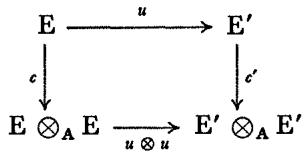
\includegraphics[keepaspectratio]{images/part004_6ed4336b.jpg}}

It is immediately verified that the identity mapping is a morphism, that the composition of two morphisms is a morphism and that every bijective morphism is an isomorphism.

Examples. (1) The canonical isomorphism \(\mathbf{A} \to \mathbf{A} \otimes_{\mathbf{A}} \mathbf{A}\) (II, § 3, no. 5) defines an A-cogebra structure on \(\mathbf{A}\) .

\begin{enumerate}
\def\labelenumi{(\arabic{enumi})}
\setcounter{enumi}{1}
\item
  Let E be a cogebra, c its coproduct and \(\sigma\) the canonical automorphism of the A-module \(E \otimes_{A} E\) such that \(\sigma(x \otimes y) = y \otimes x\) for \(x \in E\) , \(y \in E\) ; the A-linear mapping \(\sigma \circ c\) defines a new cogebra structure on E. With this structure E is called the opposite cogebra to the given cogebra E.
\item
  Let B be an A-algebra and let \(m:B \otimes_{A} B \to B\) be the A-linear mapping defining multiplication on B ( \(\S 1\) , no. 3). The transpose \(^{t}m\) is then an A-linear mapping of the dual \(B^{*}\) of the A-module B into the dual \((\mathbf{B} \otimes_{\mathbf{A}} \mathbf{B})^{*}\) of the A-module \(B \otimes_{A} B\) . If also B is a finitely generated projective A-module, the canonical mapping \(\mu:B^{*} \otimes_{A} B^{*} \to (\mathbf{B} \otimes_{\mathbf{A}} \mathbf{B})^{*}\) is an A-module isomorphism (II, \(\S 4\) , no. 4); the mapping \(c = \mu^{-1} \circ ^{t}m\) is then a coproduct defining a cogebra structure on the dual \(B^{*}\) of the A-module B.
\item
  Let X be a set, \(\mathbf{A}^{(\mathbf{X})}\) the A-module of formal linear combinations of elements of X with coefficients in A (II, §1, no. 11) and \((e_{x})_{x\in\mathbf{X}}\) the canonical basis of \(\mathbf{A}^{(\mathbf{X})}\) . An A-linear mapping \(c:A^{(\mathbf{X})}\to\mathbf{A}^{(\mathbf{X})}\otimes_{\mathbf{A}}\mathbf{A}^{(\mathbf{X})}\) is defined by the condition \(c(e_{x})=e_{x}\otimes e_{x}\) and a canonical cogebra structure is thus obtained on \(\mathbf{A}^{(\mathbf{X})}\) .
\item
  Let \(\mathbf{M}\) be an A-module and \(\mathsf{T}(\mathbf{M})\) the tensor algebra of \(\mathbf{M}\) ( \(\S 5\) , no. 1); by II, \(\S 3\) , no. 9 there exists one and only one A-linear mapping \(c\) of the A-module \(\mathsf{T}(\mathbf{M})\) into the A-module \(\mathsf{T}(\mathbf{M}) \otimes_{\mathbf{A}} \mathsf{T}(\mathbf{M})\) such that, for all \(n \geqslant 0\) ,
\end{enumerate}

\[
c (x _ {1} x _ {2} \dots x _ {n}) = \sum_ {0 \leqslant p \leqslant n} (x _ {1} x _ {2} \dots x _ {p}) \otimes (x _ {p + 1} \dots x _ {n})\tag{3}
\]

for all \(x_{i} \in \mathbf{M}\) ( \(x_{1}x_{2}\ldots x_{n}\) denotes the product in the algebra \(\mathsf{T}(\mathbf{M})\) ). Thus \(\mathsf{T}(\mathbf{M})\) is given a cogebra structure.

\begin{enumerate}
\def\labelenumi{(\arabic{enumi})}
\setcounter{enumi}{5}
\tightlist
\item
  Let M be an A-module and S(M) the symmetric algebra of M (§ 6, no. 1); the diagonal mapping \(\Delta: x \mapsto (x, x)\) of M into M × M is an A-linear mapping to which there therefore corresponds a homomorphism S(Δ) of the A-algebra S(M) into the A-algebra S(M × M) (§ 6, no. 2, Proposition 3). On the other hand, in § 6, no. 6 we defined a canonical graded algebra isomorphism \(h \colon \mathbb{S}(\mathbf{M} \times \mathbf{M}) \to \mathbb{S}(\mathbf{M}) \otimes_{\mathbf{A}} \mathbb{S}(\mathbf{M})\) ; by composition we therefore obtain an A-algebra homomorphism
\end{enumerate}

\[
c = h \circ \mathbf {S} (\Delta): \mathbf {S} (\mathbf {M}) \rightarrow \mathbf {S} (\mathbf {M}) \otimes_ {\mathbf {A}} \mathbf {S} (\mathbf {M}),
\]

thus defining on \(\mathbf{S}(\mathbf{M})\) a cogebra structure. For all \(x\in \mathbf{M}\) , by definition \(\mathbf{S}(\Delta)(x) = (x,x)\) and the definition of \(h\) given in § 6, no. 6 shows that

\[
h ((x, x)) = x \otimes 1 + 1 \otimes x.
\]

It follows that \(c\) is the unique algebra homomorphism such that, for all \(x \in \mathbf{M}\) ,

\[
c (x) = x \otimes 1 + 1 \otimes x.\tag{4}
\]

As \(c\) is an algebra homomorphism, it follows that, for every sequence \((x_{i})_{1\leqslant i\leqslant n}\) of \(n\) elements of \(\mathbf{M}\) ,

\[
\begin{array}{r l} c (x _ {1} x _ {2} \dots x _ {n}) & = \prod_ {i = 1} ^ {n} (x _ {i} \otimes 1 + 1 \otimes x _ {i}) \\ & = \sum (x _ {i _ {1}} \dots x _ {i _ {p}}) \otimes (x _ {j _ {1}} \dots x _ {j _ {n - p}}) \end{array}\tag{5}
\]

the summation on the right hand side of (5) being taken over all ordered pairs of strictly increasing sequences (in some cases empty)

\[
i _ {1} <   i _ {2} <   \dots <   i _ {p}, \quad j _ {1} <   j _ {2} <   \dots <   j _ {n - p}
\]

of elements of \([1, n]\) , whose sets of elements are complementary. The element \(c(x_1 x_2 \ldots x_n)\) is an element of total degree \(n\) in \(\mathbb{S}(\mathbf{M}) \otimes_{\mathbf{A}} \mathbb{S}(\mathbf{M})\) and its component of bidegree \((p, n - p)\) is

\[
\sum_ {\sigma} \left(x _ {\sigma (1)} \dots x _ {\sigma (p)}\right) \otimes \left(x _ {\sigma (p + 1)} \dots x _ {\sigma (n)}\right)\tag{6}
\]

where the summation is taken over all permutations \(\sigma\in\mathbb{S}_{n}\) which are increasing in each of the intervals \([1,p]\) and \([p+1,n]\) .

\begin{enumerate}
\def\labelenumi{(\arabic{enumi})}
\setcounter{enumi}{6}
\tightlist
\item
  Let \(\mathbf{M}\) be an A-module and proceed with the exterior algebra \(\bigwedge (\mathbf{M})\) as with \(\mathbb{S}(\mathbf{M})\) in Example 6; the diagonal mapping \(\Delta : \mathbf{M} \to \mathbf{M} \times \mathbf{M}\) this time defines a homomorphism \(\bigwedge (\Delta)\) of the A-algebra \(\bigwedge (\mathbf{M})\) into the A-algebra \(\bigwedge (\mathbf{M} \times \mathbf{M})\) (§ 7, no. 2, Proposition 2); on the other hand there is a canonical graded algebra isomorphism
\end{enumerate}

\[
h: \bigwedge (\mathbf {M} \times \mathbf {M}) \rightarrow \bigwedge (\mathbf {M}) ^ {\mathrm{g}} \otimes_ {\mathbf {A}} \bigwedge (\mathbf {M})
\]

(§ 7, no. 7, Proposition 10), whence by composition there is an algebra homomorphism \(c = h \circ \bigwedge(\Delta): \bigwedge(M) \to \bigwedge(M)^{\mathfrak{g}} \otimes_{A} \bigwedge(M)\) , which can be considered as an A-module homomorphism \(\bigwedge(M) \to \bigwedge(M) \otimes_{A} \bigwedge(M)\) and which therefore defines on \(\bigwedge(M)\) a cogebra structure. It can be proved as in Example 6 that \(c\) is the unique algebra homomorphism such that, for all \(x \in M\) ,

\[
c (x) = x \otimes 1 + 1 \otimes x,\tag{7}
\]

whence, for every sequence \((x_{i})_{1\leqslant i\leqslant n}\) of elements of \(\mathbf{M}\) ,

\[
c \left(x _ {1} \wedge x _ {2} \wedge \dots \wedge x _ {n}\right) = \left(x _ {1} \otimes 1 + 1 \otimes x _ {1}\right) \wedge \dots \wedge \left(x _ {n} \otimes 1 + 1 \otimes x _ {n}\right)
\]

where the product on the right hand side is taken in the algebra

\[
\Lambda (\mathbf {M}) ^ {\mathfrak {g}} \otimes_ {\mathbf {A}} \Lambda (\mathbf {M});
\]

to calculate this product, consider, for every ordered pair of strictly increasing sequences \(i_1 < i_2 < \cdots < i_p\) , \(j_1 < j_2 < \cdots < j_{n-p}\) of elements of \([1, n]\) , whose sets of elements are complementary, the product \(y_1y_2\ldots y_n\) , where \(y_{i_h} = x_{i_h} \otimes 1 (1 \leqslant h \leqslant p)\) and \(y_{j_k} = 1 \otimes x_{j_k} (1 \leqslant k \leqslant n - p)\) and the sum is taken over all these products. As the graded algebra \(\bigwedge (\mathbf{M})^{\mathfrak{g}} \otimes_{\mathbf{A}} \bigwedge (\mathbf{M})\) is anticommutative and the elements \(x_i \otimes 1\) and \(1 \otimes x_i\) are of total degree 1, by §4, no. 6, Lemma 3 and Lemma 1,

\[
\begin{array}{r l} c (x _ {1} \wedge x _ {2} \wedge \dots \wedge x _ {n}) & = \sum (- 1) ^ {\nu} (x _ {i _ {1}} \wedge \dots \wedge x _ {i _ {p}}) \otimes (x _ {j _ {1}} \wedge \dots \wedge x _ {j _ {n - p}}) \end{array} \tag {8}
\]

v being the number of ordered pairs \((h, k)\) such that \(j_{k} < i_{h}\) and the summation being taken over the same set as in (5). The element \(c(x_{1} \wedge \cdots \wedge x_{n})\) is of total degree n in \(\bigwedge(\mathbf{M})^{\mathbf{g}} \otimes_{\mathbf{A}} \bigwedge(\mathbf{M})\) and its homogeneous component of bi-degree \((p, n - p)\) is equal to

\[
\sum_ {\sigma} \varepsilon_ {\sigma} (x _ {\sigma (1)} \wedge \dots \wedge x _ {\sigma (p)}) \otimes (x _ {\sigma (p + 1)} \wedge \dots \wedge x _ {\sigma (n)})\tag{9}
\]

the summation being taken over permutations \(\sigma\in\mathfrak{S}_{n}\) which are increasing in each of the intervals \([1,p]\) and \([p+1,n]\) .

When in future we speak of \(\mathbf{A}^{(\mathbf{X})}\) , \(\mathsf{T}(\mathbf{M})\) , \(\mathsf{S}(\mathbf{M})\) or \(\bigwedge (\mathbf{M})\) as cogebras, we shall mean, unless otherwise mentioned, with the cogebra structures defined in Examples 4, 5, 6 and 7 respectively.

\begin{enumerate}
\def\labelenumi{(\arabic{enumi})}
\setcounter{enumi}{7}
\tightlist
\item
  Let E, F be two A-cogebras and c, \(c'\) their respective coproducts. Let \(\tau:(\mathbf{E} \otimes_{\mathbf{A}} \mathbf{E}) \otimes_{\mathbf{A}} (\mathbf{F} \otimes_{\mathbf{A}} \mathbf{F}) \to (\mathbf{E} \otimes_{\mathbf{A}} \mathbf{F}) \otimes_{\mathbf{A}} (\mathbf{E} \otimes_{\mathbf{A}} \mathbf{F})\) denote the associativity isomorphism such that \(\tau((x \otimes x') \otimes (y \otimes y')) = (x \otimes y) \otimes (x' \otimes y')\) for \(x, x'\) in E and \(y, y'\) in F. Then the composite linear mapping
\end{enumerate}

\[
\mathrm{E} \otimes_ {\mathrm{A}} \mathrm{F} \xrightarrow {c \otimes c ^ {\prime}} (\mathrm{E} \otimes_ {\mathrm{A}} \mathrm{E}) \otimes_ {\mathrm{A}} (\mathrm{F} \otimes_ {\mathrm{A}} \mathrm{F}) \xrightarrow {\tau} (\mathrm{E} \otimes_ {\mathrm{A}} \mathrm{F}) \otimes_ {\mathrm{A}} (\mathrm{E} \otimes_ {\mathrm{A}} \mathrm{F})
\]

defines a cogebra structure on the A-module E \(\otimes_{\mathbf{A}}\mathbf{F}\) , called the tensor product of the cogebras E and F.

Let E be a cogebra and \(\Delta\) a commutative monoid. A graduation \((\mathrm{E}_{\lambda})_{\lambda\in\Delta}\) on the A-module E is said to be compatible with the coproduct c of E if c is a graded homomorphism of degree 0 of the graded A-module E into the graded A-module (of type \(\Delta\) ) \(E\otimes_{A}E\) , in other words (II, §11, no. 5) if

\[
\mathrm{c} (\mathrm{E} _ {\lambda}) \subset \sum_ {\mu + \nu = \lambda} \mathrm{E} _ {\mu} \otimes_ {\mathbf {A}} \mathrm{E} _ {\nu}.\tag{10}
\]

In what follows, we shall most often limit our attention to graduations of type N compatible with the coproduct; a cogebra with such a graduation will also be called a graded cogebra. If F is another graded cogebra, a graded cogebra morphism \(\phi:E\to F\) is by definition a cogebra morphism (Definition 2) which is also a graded homomorphism of degree 0 of graded A-modules.

Examples. (9) It is immediate that the cogebras \(\mathsf{T}(\mathbf{M})\) , \(\mathsf{S}(\mathbf{M})\) and \(\bigwedge (\mathbf{M})\) defined above are graded cogebras.

\subsection{COASSOCIATIVITY, COCOMMUTATIVITY, COUNIT}

Let E be a cogebra, c its coproduct, N, N', N'' three A-modules and m a bilinear mapping of N × N' into N''. Let \(\tilde{m}:N \otimes_{A} N' \to N''\) denote the A-linear mapping corresponding to m. If \(u:E \to N\) , \(v:E \to N'\) are two A-linear mappings, we derive an A-linear mapping \(u \otimes v:E \otimes_{A} E \to N \otimes_{A} N'\) and a composite A-linear mapping of E into N'':

\[
m (u, v): \mathrm{E} \xrightarrow {c} \mathrm{E} \otimes_ {\mathrm{A}} \mathrm{E} \xrightarrow {u \otimes v} \mathrm{N} \otimes_ {\mathrm{A}} \mathrm{N} ^ {\prime} \xrightarrow {\tilde {m}} \mathrm{N} ^ {\prime \prime}.\tag{11}
\]

Clearly we have thus defined an A-bilinear mapping \((u, v) \mapsto m(u, v)\) of \(\operatorname{Hom}_{\mathbf{A}}(\mathbf{E}, \mathbf{N}) \times \operatorname{Hom}_{\mathbf{A}}(\mathbf{E}, \mathbf{N}')\) into \(\operatorname{Hom}_{\mathbf{A}}(\mathbf{E}, \mathbf{N}'')\) .

When E is a graded cogebra, N, N', N'' graded A-modules of the same type and \(\tilde{m}\) a graded homomorphism of degree k of N \(\otimes_{A}N'\) into N'', then, if u (resp. v) is a graded homomorphism of degree p (resp. q), \(m(u,v)\) is a graded homomorphism of degree \(p + q + k\) .

Examples. (1) Take E to be the graded cogebra T(M) (no. 1) and suppose that N, N', N'' have the trivial graduation. A graded homomorphism of degree -p of T(M) into N (resp. N', N'') then corresponds to a multilinear mapping of M\^{}p into N (resp. N', N''). Given a multilinear mapping u: M\^{}p → N and a multilinear mapping v: M\^{}q → N', the above method allows us to deduce a multilinear mapping m(u, v): M\^{}\{p+q\} → N'' called the product (relative to m) of u and v. Formulae (3) (no. 1) and (11) show that, for x\_1, . . ., x\_p+q in M,

\[
(m (u, v)) \left(x _ {1}, \dots , x _ {p + q}\right) = m \left(u \left(x _ {1}, \dots , x _ {p}\right), v \left(x _ {p + 1}, \dots , x _ {p + q}\right)\right).
\]

\begin{enumerate}
\def\labelenumi{(\arabic{enumi})}
\setcounter{enumi}{1}
\tightlist
\item
  Take E to be the graded cogebra S(M) (no. 1), preserving the same hypotheses on N, N', N''. A graded homomorphism of degree -p of S(M) into N then corresponds to a symmetric multilinear mapping of M \(^{p}\) into N (§ 6, no. 3). Then we derive from a symmetric multilinear mapping u: M \(^{p}\) → N and a symmetric multilinear mapping v: M \(^{q}\) → N' a symmetric multilinear mapping m(u, v): M \(^{p+q}\) → N'', also denoted (to avoid confusion) by \(u \cdot_{m} v\) (or even \(u \cdot v\)) and called the symmetric product (relative to m) of u and v. Formulae (6) (no. 1) and (11) show that, for x₁, \ldots, x \(_{p+q}\) in M,
\end{enumerate}

\[
(u \cdot_{m} v) (x _ {1}, \dots , x _ {p + q}) = \sum_ {\sigma} m (u (x _ {\sigma (1)}, \dots , x _ {\sigma (p)}), v (x _ {\sigma (p + 1)}, \dots , x _ {\sigma (p + q)}))
\]

the summation being taken over permutations \(\sigma\in\mathfrak{S}_{p+q}\) which are increasing on each of the intervals \([1,p]\) and \([p+1,p+q]\) .

\begin{enumerate}
\def\labelenumi{(\arabic{enumi})}
\setcounter{enumi}{2}
\tightlist
\item
  Take E to be the graded cogebra \(\bigwedge (\mathbf{M})\) (no. 1). Then we deduce similarly from an alternating multilinear mapping \(u: \mathbf{M}^p \to \mathbf{N}\) and an alternating multilinear mapping \(v: \mathbf{M}^q \to \mathbf{N}'\) an alternating multilinear mapping \(m(u, v): \mathbf{M}^{p + q} \to \mathbf{N}''\) , also denoted by \(u \wedge_m v\) or \(u \wedge v\) and called the alternating product (relative to \(m\) ) of \(u\) and \(v\) . Formulae (9) (no. 1) and (11) show in this case that, for \(x_1, \ldots, x_{p + q}\) in \(\mathbf{M}\) ,
\end{enumerate}

\[
(u \wedge_ {m} v) (x _ {1}, \dots , x _ {p + q}) = \sum_ {\sigma} \varepsilon_ {\sigma} m (u (x _ {\sigma (1)}, \dots , x _ {\sigma (p)}), v (x _ {\sigma (p + 1)}, \dots , x _ {\sigma (p + q)}))
\]

the summation again being taken over permutations \(\sigma \in \mathfrak{S}_{p + q}\) which are increasing on each of the intervals \([1, p]\) and \([p + 1, p + q]\) .

We return to the case where E is an arbitrary graded cogebra (of type N) and assume that the three modules N, N', N'' are all equal to the underlying A-module of a graded A-algebra B of type Z, the mapping m being multiplication in B, so that \(\tilde{m}:B\otimes_{A}B\to B\) is a graded A-linear mapping of degree 0. Thus a graded A-algebra structure is obtained on the graded A-module \(\operatorname{Homgr}_{A}(E,B)=C\) .

In particular, suppose that B = A (with the trivial graduation), so that \(\operatorname{Homgr}_{\mathbf{A}}(\mathbf{E}, \mathbf{A})\) is the graded dual \(E^{*gr}\) , which thus has a graded A-algebra structure.

Let F be another graded cogebra \(c'\) its coproduct and \(\phi:E\to F\) a graded cogebra morphism (no. 1); then the canonical graded morphism

\[
\tilde {\phi} = \operatorname{Hom} (\phi , 1 _ {B}): \operatorname{Homgr} _ {A} (F, B) \rightarrow \operatorname{Homgr} _ {A} (E, B)
\]

is a graded algebra homomorphism. For \(u, v\) in \(\operatorname{Homgr}_{\mathbf{A}}(\mathbf{F}, \mathbf{B})\) and \(x \in \mathbf{E}\) ,

\[
(\tilde {\phi} (u v)) (x) = (u v) (\phi (x)) = m ((u \otimes v) (c ^ {\prime} (\phi (x))))
\]

But by hypothesis \(c'(\phi(x)) = (\phi \otimes \phi)(c(x))\) , hence

\[
(u \otimes v) (c ^ {\prime} (\phi (x))) = (\tilde {\phi} (u) \otimes \tilde {\phi} (v)) (c (x))
\]

and therefore \(\tilde{\phi}(uv) = \tilde{\phi}(u)\tilde{\phi}(v)\) , which proves our assertion.

In particular, the graded transpose \({}^{t}\phi: \mathrm{F}^{*gr} \to \mathrm{E}^{*gr}\) is a graded algebra homomorphism.

Remark. Suppose that the \(E_{p}\) are finitely generated projective A-modules, so that the graded A-modules ( \(E \otimes_{A} E)^{*gr}\) and \(E^{*gr} \otimes_{A} E^{*gr}\) can be canonically identified (II, §4, no. 4, Corollary 1 to Proposition 4). If also the A-modules \(A \otimes_{A} A\) and A are then canonically identified (II, §3, no. 4), the linear mapping \(E^{*gr} \otimes_{A} E^{*gr} \to E^{*gr}\) which defines multiplication in \(E^{*gr}\) can be called the graded transpose of the coproduct c.

PROPOSITION 1. Let E be a cogebra over A. In order that, for every associative A-algebra B, the A-algebra \(\operatorname{Hom}_{\mathbf{A}}(\mathbf{E}, \mathbf{B})\) be associative, it is necessary and sufficient that the coproduct \(c: \mathbf{E} \to \mathbf{E} \otimes_{\mathbf{A}} \mathbf{E}\) be such that the diagram

\begin{enumerate}
\def\labelenumi{(\arabic{enumi})}
\setcounter{enumi}{11}
\tightlist
\item
\end{enumerate}

\pandocbounded{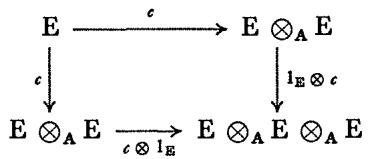
\includegraphics[keepaspectratio]{images/part004_a79ed2ff.jpg}}

be commutative.

Let B be an associative A-algebra and u, v, w three elements of \(\mathbf{C} = \operatorname{Hom}_{\mathbf{A}}(\mathbf{E}, \mathbf{B})\) . Let \(m_{3}\) denote the A-linear mapping \(B \otimes_{A} B \otimes_{A} B \to B\) which maps \(b \otimes b' \otimes b''\) to \(bb'b''\) . By definition of the product on the algebra C, \((uv)w\) is the composite mapping

\[
\mathrm{E} \xrightarrow {c} \mathrm{E} \otimes \mathrm{E} \xrightarrow {c \otimes 1 _ {\mathrm{E}}} \mathrm{E} \otimes \mathrm{E} \otimes \mathrm{E} \xrightarrow {u \otimes v \otimes w} \mathrm{B} \otimes \mathrm{B} \otimes \mathrm{B} \xrightarrow {m _ {3}} \mathrm{B}
\]

whilst \(u(vw)\) is the composite mapping

\[
\mathrm{E} \xrightarrow {c} \mathrm{E} \otimes \mathrm{E} \xrightarrow {1 _ {\mathrm{E}} \otimes c} \mathrm{E} \otimes \mathrm{E} \otimes \mathrm{E} \xrightarrow {u \otimes v \otimes w} \mathrm{B} \otimes \mathrm{B} \otimes \mathrm{B} \xrightarrow {m _ {3}} \mathrm{B}.
\]

It follows that if diagram (12) is commutative, the algebra \(\operatorname{Hom}_{\mathbf{A}}(\mathbf{E}, \mathbf{B})\) is associative for every associative A-algebra B. To establish the converse, it suffices to show that there exists an associative A-algebra B and three A-linear mappings \(u, v, w\) of E into B such that the mapping \(m_3 \circ (u \otimes v \otimes w)\) of \(\mathbf{E} \otimes \mathbf{E} \otimes \mathbf{E}\) into B is injective. Take B to be the A-algebra \(\mathsf{T}(\mathbf{E})\) and \(u, v, w\) the canonical mapping of E into \(\mathsf{T}(\mathbf{E})\) . The mapping \(m_3 \circ (u \otimes v \otimes w)\) is then the canonical mapping \(\mathbf{E} \otimes \mathbf{E} \otimes \mathbf{E} = \mathsf{T}^3(\mathbf{E}) \to \mathsf{T}(\mathbf{E})\) , which is injective.

When the cogebra E satisfies the condition of Proposition 1, it is said to be coassociative.

Examples. (4) It is immediately verified that the cogebra A (no. 1, Example (1)) the cogebra \(\mathbf{A}^{(\mathbf{X})}\) (no. 1, Example 4) and the cogebra \(\mathbf{T}(\mathbf{M})\) (no. 1, Example 5) are coassociative. If B is an associative A-algebra which is a finitely generated projective A-module, the cogebra \(\mathbf{B}^*\) (no. 1, Example 3) is coassociative: for the commutativity of diagram (12) then follows by transposition from that of the diagram which expresses the associativity of B ( \(\S\) 1, no. 3). Conversely, the same argument and the canonical identification of the A-module B with its bidual (II, § 2, no. 7, Corollary 4 to Proposition 13) show that if the cogebra \(\mathbf{B}^*\) is coassociative, the algebra \(\mathbf{B}\) is associative. Finally, the cogebras \(\mathsf{S}(\mathbf{M})\) and \(\bigwedge (\mathbf{M})\) (no. 1, Examples 6 and 7) are coassociative; this follows from the commutativity of the diagram

\[
\begin{array}{c} \mathrm{M} \xrightarrow {\Delta} \mathrm{M} \times \mathrm{M} \\ \Delta \Biggl \downarrow \\ \mathrm{M} \times \mathrm{M} \xrightarrow [ \Delta \times 1 _ {\mathrm{M}} ]{} \mathrm{M} \times \mathrm{M} \times \mathrm{M} \end{array}
\]

the functorial properties of \(\mathsf{S}(\mathbf{M})\) ( \(\S 6\) , no. 2) and \(\bigwedge (\mathbf{M})\) ( \(\S 7\) , no. 2), which give the corresponding commutative diagrams

\[
\left\{ \begin{array}{c} \mathsf {S} (\mathbf {M}) \xrightarrow {\mathsf {S} (\Delta)} \mathsf {S} (\mathbf {M} \times \mathbf {M}) \\ \mathsf {S} (\Delta) \Biggl \downarrow \qquad \qquad \qquad \qquad \qquad \qquad \qquad \qquad \qquad \qquad \qquad \qquad \qquad \qquad \qquad \qquad \qquad \qquad \qquad \qquad \qquad \qquad \qquad \qquad \qquad \qquad \qquad \qquad \qquad \qquad \qquad \qquad \qquad \qquad \mathsf {S} (1 _ {\mathbf {M}} \times \Delta) \\ \mathsf {S} (\mathbf {M} \times \mathbf {M}) \xrightarrow [ \mathsf {S} (\Delta \times 1 _ {\mathbf {M}}) ]{\mathsf {S} (\Delta \times 1 _ {\mathbf {M}})} \mathsf {S} (\mathbf {M} \times \mathbf {M} \times \mathbf {M}) \\ \bigwedge (\mathbf {M}) \xrightarrow {\bigwedge (\Delta)} \bigwedge (\mathbf {M} \times \mathbf {M}) \\ \bigwedge (\Delta) \Biggl \downarrow \qquad \qquad \qquad \qquad \qquad \qquad \qquad \qquad \qquad \qquad \qquad \qquad \qquad \bigwedge (1 _ {\mathbf {M}} \times \Delta) \\ \bigwedge (\mathbf {M} \times \mathbf {M}) \xrightarrow [ \bigwedge (\Delta \times 1 _ {\mathbf {M}}) ]{\bigwedge (\Delta \times 1 _ {\mathbf {M}})} \bigwedge (\mathbf {M} \times \mathbf {M} \times \mathbf {M}) \end{array} \right.\tag{14}
\]

and the existence and functoriality of canonical isomorphisms for symmetric and exterior algebras of a direct sum (§ 6, no. 6 and § 7, no. 7).

PROPOSITION 2. Let E be a cogebra over A. In order that, for every commutative A-algebra B, the A-algebra \(\operatorname{Hom}_{\mathbf{A}}(\mathbf{E}, \mathbf{B})\) be commutative, it is necessary and sufficient that the coproduct \(c: \mathbf{E} \to \mathbf{E} \otimes_{\mathbf{A}} \mathbf{E}\) be such that the diagram

\begin{enumerate}
\def\labelenumi{(\arabic{enumi})}
\setcounter{enumi}{14}
\tightlist
\item
\end{enumerate}

\pandocbounded{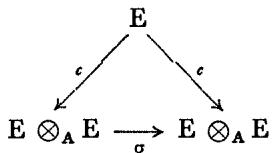
\includegraphics[keepaspectratio]{images/part004_07c99209.jpg}}

(where \(\sigma\) is the symmetry homomorphism such that \(\sigma(x \otimes y) = y \otimes x\) ) is commutative (in other words, it suffices that the cogebra E be identical with its opposite (no. 1, Example 2).

Let B be a commutative A-algebra and u, v two elements of C = Hom\_A(E, B).

By definition of the product in C, uv and vu are respectively equal to the composite mappings

\[
\mathrm{E} \xrightarrow {c} \mathrm{E} \otimes \mathrm{E} \xrightarrow {u \otimes v} \mathrm{B} \otimes \mathrm{B} \xrightarrow {m} \mathrm{B}
\]

and

\[
\mathrm{E} \xrightarrow {c} \mathrm{E} \otimes \mathrm{E} \xrightarrow {v \otimes u} \mathrm{B} \otimes \mathrm{B} \xrightarrow {m} \mathrm{B}.
\]

It follows that if diagram (15) is commutative the algebra \(\operatorname{Hom}_{\mathbf{A}}(\mathbf{E}, \mathbf{B})\) is commutative for every commutative A-algebra B. To establish the converse, it suffices to show that there exist a commutative A-algebra B and two A-linear mappings \(u, v\) of E into B such that \(m \circ (u \otimes v): \mathbf{E} \otimes \mathbf{E} \to \mathbf{B}\) is injective. Take B to be the algebra \(\mathsf{S}(\mathbf{E} \oplus \mathbf{E})\) and \(u\) (resp. \(v\) ) the composition of the canonical mapping \(\mathbf{E} \oplus \mathbf{E} \to \mathsf{S}(\mathbf{E} \oplus \mathbf{E})\) and the mapping \(x \mapsto (x, 0)\) (resp. \(x \mapsto (0, x)\) ) of E into \(\mathbf{E} \oplus \mathbf{E}\) . If \(h: \mathsf{S}(\mathbf{E}) \otimes \mathsf{S}(\mathbf{E}) \to \mathsf{S}(\mathbf{E} \otimes \mathbf{E})\) is the canonical isomorphism ( \(\S 6\) , no. 6, Proposition 9) and \(\lambda: \mathbf{E} \to \mathsf{S}(\mathbf{E})\) is the canonical mapping, then \(h^{-1} \circ m \circ (u \otimes v) = \lambda \otimes \lambda\) . Now \(\lambda \otimes \lambda\) is injective, for \(\lambda(\mathbf{E})\) is a direct factor of \(\mathsf{S}(\mathbf{E})\) (II, § 3, no. 7, Corollary 5 to Proposition 7).

When the cogebra E satisfies the condition of Proposition 2, it is said to be cocommutative.

Examples. (5) It is immediate that the cogebra A (no. 1, Example 1) and the cogebra \(\mathbf{A}^{(\mathbf{X})}\) (II, § 11, no. 1, Example 4) are cocommutative. It follows from formula (5) of no. 1 that the cogebra S(M) is cocommutative. Finally, for an A-algebra B such that the A-module B is projective and finitely generated to have the property that the cogebra \(\mathbf{B}^*\) (no. 1, Example 3) is cocommutative, it is necessary and sufficient that B be commutative; for (using the canonical identification of the A-module B with its bidual (II, § 2, no. 7)), this follows from the fact that the commutativity of diagram (14) is equivalent by transposition to that of the diagram which expressed the commutativity of B (§ 1, no. 3).

PROPOSITION 3. Let E be a cogebra over A. In order that, for every unital A-algebra B, the A-algebra \(\operatorname{Hom}_{\mathbf{A}}(\mathbf{E},\mathbf{B})\) be unital, it is necessary and sufficient that there exist a linear form \(\gamma\) on E rendering commutative the diagrams

\begin{enumerate}
\def\labelenumi{(\arabic{enumi})}
\setcounter{enumi}{15}
\tightlist
\item
\end{enumerate}

\pandocbounded{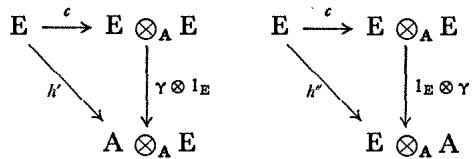
\includegraphics[keepaspectratio]{images/part004_cc0e83d1.jpg}}

where \(c: \mathbf{E} \to \mathbf{E} \otimes_{\mathbf{A}} \mathbf{E}\) is the coproduct and \(h'\) and \(h''\) the canonical isomorphisms (II, § 3, no. 4, Proposition 4). The unit of \(\operatorname{Hom}_{\mathbf{A}}(\mathbf{E}, \mathbf{B})\) is then the linear mapping \(x \mapsto \gamma(x)1\) (where 1 denotes the unit element of B).

Let \(\gamma\) be a linear form on E rendering diagram (16) commutative. Let B be a unital A-algebra with unit element 1, \(\eta: \mathbf{A} \to \mathbf{B}\) the canonical mapping and \(v = \eta \circ \gamma\) the element of the A-algebra \(\mathbf{C} = \operatorname{Hom}_{\mathbf{A}}(\mathbf{E}, \mathbf{B})\) . For every element \(u \in \mathbf{C}\) , \(uv\) is the composite mapping

\[
\mathrm{E} \xrightarrow {c} \mathrm{E} \otimes \mathrm{E} \xrightarrow {1 _ {\mathrm{E}} \otimes \gamma} \mathrm{E} \otimes \mathrm{A} \xrightarrow {u \otimes \eta} \mathrm{B} \otimes \mathrm{B} \xrightarrow {m} \mathrm{B}.\tag{17}
\]

Then \(uv = m \circ (u \otimes \eta) \circ h'' = u\) . It is similarly proved that \(vu = u\) and hence \(v\) is unit element of C. Conversely, let the A-module A ⊕ E be given a unital algebra structure such that \((a, x)(a', x') = (aa', ax' + a'x)\) for \(a, a'\) in A and \(x, x'\) in E. Let B denote the A-algebra thus defined and let C be the A-algebra Hom \(_A(E, B)\) . Suppose that C is unital and let \(e: x \mapsto (\gamma(x), \lambda(x))\) be its unit element (where \(\gamma(x) \in A\) and \(\lambda(x) \in E\) ). On the other hand let \(f\) be the element \(x \mapsto (0, x)\) of C. An immediate calculation shows that \(fe\) is the element

\[
x \mapsto (0, (h ^ {\prime \prime}) ^ {- 1} ((1 _ {E} \otimes \gamma) (c (x))))
\]

of C. The condition \(fe = f\) implies the commutativity of the second diagram of (16) and it is similarly seen that the condition \(ef = f\) implies the commutativity of the first diagram of (16).

A linear form \(\gamma\) on E rendering diagrams (16) commutative is called a counit of the cogebra E. A cogebra admits at most one counit: for it is the unit element of the algebra \(\operatorname{Hom}_{\mathbf{A}}(\mathbf{E}, \mathbf{A})\) . A cogebra with a counit is called counital.

Examples. (6) The identity mapping is the counit of the cogebra A; on the cogebra \(\mathbf{A}^{(\mathbf{X})}\) (no. 1, Example 4) the linear form \(\gamma\) such that \(\gamma(e_x) = 1\) for all \(x \in \mathbf{X}\) is the counit. On the cogebra \(\mathbf{T}(\mathbf{M})\) (resp. \(\mathbf{S}(\mathbf{M}), \bigwedge(\mathbf{M})\) ) the linear form \(\gamma\) such that \(\gamma(1) = 1\) and \(\gamma(z) = 0\) for \(z\) in the \(\mathbf{T}^n(\mathbf{M})\) (resp. \(\mathbf{S}^n(\mathbf{M}), \bigwedge^n(\mathbf{M})\) ) for \(n \geqslant 1\) is the counit. Finally, let B be an A-algebra which is a finitely generated projective A-module and has a unit element \(e\) ; then on the cogebra \(\mathbf{B}^*\) (no. 1, Example 3) the linear form \(\gamma: x^* \mapsto \langle e, x^* \rangle\) is the counit, for this form is just the transpose of the A-linear mapping \(\eta_e: \xi \mapsto \xi e\) of A into B and by transposition the commutativity of diagrams (16) follows from that of the diagrams which express (using \(\eta_e\) ) the fact that \(e\) is unit element of B ( \(\S 1\) , no. 3); the same argument moreover shows that conversely, if the cogebra \(\mathbf{B}^*\) admits a counit \(\gamma\) , the transpose of \(\gamma\) defines a unit element \(e = {}^t\gamma(1)\) of B.

PROPOSITION 4. Let E be a cogebra admitting a counit \(\gamma\) and suppose that there exists in E an element \(e\) such that \(\gamma(e) = 1\) ; then E is the direct sum of the sub-A-modules Ae and \(\mathrm{E}_{\gamma} = \mathrm{Ker}(\gamma)\) and

\[
c (e) \equiv e \otimes e (\mathrm{mod.} \mathrm{E} _ {\gamma} \otimes \mathrm{E} _ {\gamma})\tag{18}
\]

\[
\left\{c (x) \equiv x \otimes e + e \otimes x (\mathrm{mod.} \mathrm{E} _ {\gamma} \otimes \mathrm{E} _ {\gamma}) \quad \text { for all } x \in \mathrm{E} _ {\gamma}. \right.
\]

The first assertion is immediate, for \(\gamma(x - \gamma(x)e) = 0\) and the relation \(\gamma(\alpha e) = 0\) implies \(\alpha = 0\) . Let \(c(e) = \sum_{i} s_i \otimes t_i\) , so that

\[
e = \sum_ {i} \gamma (s _ {i}) t _ {i} = \sum_ {i} \gamma (t _ {i}) s _ {i}
\]

by (16) and \(1 = \gamma(e) = \sum_{i} \gamma(s_i) \gamma(t_i)\) . Therefore

\[
\begin{array}{r l} \sum_ {i} (s _ {i} - \gamma (s _ {i}) e) \otimes (t _ {i} - \gamma (t _ {i}) e) & = \sum_ {i} s _ {i} \otimes t _ {i} - \sum_ {i} e \otimes \gamma (s _ {i}) t _ {i} \\ & - \sum_ {i} \gamma (t _ {i}) s _ {i} \otimes e \\ & + \sum_ {i} \gamma (s _ {i}) e \otimes \gamma (t _ {i}) e \end{array}
\]

which, by the above relation, is just \(c(e) - e \otimes e\) ; this therefore proves the first relation of (18). On the other hand the decomposition of E \(\otimes\) E as a direct sum

\[
\mathbf {A} (e \otimes e) \oplus ((\mathbf {A} e) \otimes \mathbf {E} _ {\gamma}) \oplus (\mathbf {E} _ {\gamma} \otimes (\mathbf {A} e)) \oplus (\mathbf {E} _ {\gamma} \otimes \mathbf {E} _ {\gamma})
\]

allows us to write, for \(x \in \mathbf{E}_{\gamma}\) , \(c(x) = \lambda(e \otimes e) + (e \otimes y) + (z \otimes e) + u\) where \(u = \sum_{j} v_{j} \otimes w_{j}, y, z\) and the \(v_{j}\) and \(w_{j}\) belong to \(\mathbf{E}_{\gamma}\) . The definition of the counit \(\gamma\) then gives \(x = \lambda e + y = \lambda e + z\) and, as \(\gamma(x) = 0\) , necessarily \(\lambda = 0, x = y = z\) , whence the second relation of (18).

Remark. Let C be a counital coassociative A-coalgebra, B a unital associative A-algebra and M a left B-module. The A-bilinear mapping \((b, m) \mapsto bm\) of \(B \times M\) into M defines an A-bilinear mapping

\[
\operatorname{Hom} _ {\mathbf {A}} (\mathrm{C}, \mathrm{B}) \times \operatorname{Hom} _ {\mathbf {A}} (\mathrm{C}, \mathrm{M}) \rightarrow \operatorname{Hom} _ {\mathbf {A}} (\mathrm{C}, \mathrm{M})
\]

by the general procedure described at the beginning of this no. It is immediately verified that this mapping defines on \(\operatorname{Hom}_{\mathbf{A}}(\mathbf{C}, \mathbf{M})\) a left module structure over the ring \(\operatorname{Hom}_{\mathbf{A}}(\mathbf{C}, \mathbf{B})\) .

\subsection{PROPERTIES OF GRADED COGEBRAS OF TYPE N}

PROPOSITION 5. (i) Let E be a graded cogebra admitting a counit \(\gamma\) ; then \(\gamma\) is a homogeneous linear form of degree 0.

\begin{enumerate}
\def\labelenumi{(\roman{enumi})}
\setcounter{enumi}{1}
\tightlist
\item
  Suppose further that there exists an element \(e \in \mathbf{E}\) such that \(\mathbf{E}_0 = \mathbf{A}e\) and \(\gamma(e) = 1\) . Then the kernel \(\mathbf{E}_{\gamma}\) of \(\gamma\) is equal to \(\mathbf{E}_{+} = \sum_{n \geqslant 1} \mathbf{E}_n, c(e) = e \otimes e\) and
\end{enumerate}

\[
c (x) \equiv x \otimes e + e \otimes x (\mathrm{mod.} \mathrm{E} _ {+} \otimes \mathrm{E} _ {+})\tag{19}
\]

for all \(x \in \mathbf{E}_{+}\) .

\begin{enumerate}
\def\labelenumi{(\roman{enumi})}
\tightlist
\item
  It suffices to verify that \(\gamma(x) = 0\) for \(x \in \mathbf{E}_n\) , for all \(n \geqslant 1\) . Since \(c\) is a graded homomorphism of degree 0,
\end{enumerate}

\[
c (x) = \sum_ {0 \leqslant j \leqslant n} \left(\sum_ {i} y _ {i j} \otimes z _ {i, n - j}\right)\tag{20}
\]

with, for all \(j\) such that \(0 \leqslant j \leqslant n\) , \(y_{ij}\) and \(z_{ij}\) in \(\mathbf{E}_j\) ; applying (16) (no. 2) we obtain

\[
x = \sum_ {0 \leqslant j \leqslant n} \left(\sum_ {i} \gamma (y _ {i j}) z _ {i, n - j}\right) = \sum_ {0 \leqslant j \leqslant n} \left(\sum_ {i} \gamma (z _ {i, n - j}) y _ {i j}\right),
\]

whence, equating the components of degree 0 and degree n on the two sides

\[
x = \sum_ {i} \gamma (y _ {i 0}) z _ {i n} = \sum_ {i} \gamma (z _ {i 0}) y _ {i n}
\]

\[
0 = \sum_ {i} \gamma (y _ {i n}) z _ {i 0} = \sum_ {i} \gamma (z _ {i n}) y _ {i 0}
\]

and therefore \(\gamma(x) = \sum_{i} \gamma(y_{in})\gamma(z_{i0}) = \gamma(0) = 0\) .

\begin{enumerate}
\def\labelenumi{(\roman{enumi})}
\setcounter{enumi}{1}
\tightlist
\item
  Since \(\operatorname{Ker}(\gamma)\) and \(\mathbf{E}_{+}\) are both supplementary sub-A-modules of \(Ae = E_0\) and \(\mathbf{E}_{+} \subset \operatorname{Ker}(\gamma)\) by (i), \(\mathbf{E}_{+} = \operatorname{Ker}(\gamma)\) (II, § 1, no. 8, Remark 1); the other assertions follow from Proposition 4 of no. 2.
\end{enumerate}

PROPOSITION 6. Let E be a graded cogebra over A. In order that, for every commutative A-algebra B, with the trivial graduation, the graded A-algebra of type Z Homgr \(_{A}\) (E, B) (no. 2) be anticommutative (§ 4, no. 9, Definition 7), it is necessary and sufficient that, if \(\sigma_{g}\) denotes the automorphism of the A-module E \(\otimes_{A} E\) such that

\[
\sigma_ {g} (x _ {p} \otimes x _ {q}) = (- 1) ^ {p q} x _ {q} \otimes x _ {p}
\]

for \(x_{p} \in \mathbf{E}_{p}, x_{q} \in \mathbf{E}_{q}\) , where \(p\) and \(q\) are arbitrary elements of \(\mathbf{N}\) , the diagram

\begin{enumerate}
\def\labelenumi{(\arabic{enumi})}
\setcounter{enumi}{20}
\tightlist
\item
\end{enumerate}

\pandocbounded{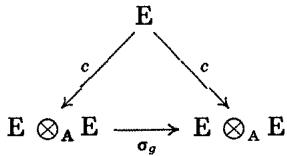
\includegraphics[keepaspectratio]{images/part004_b841500b.jpg}}

be commutative.

The proof is analogous to that of Proposition 2 of no. 2.

When the graded cogebra E satisfies the condition of Proposition 6, it is said to be anticocommutative.

Example. It follows immediately from formula (8) of no. 1 that for every A-module M, the graded cogebra \(\bigwedge(M)\) is anticocommutative.

\subsection{BIGEBRAS AND SKEW-BIGEBRAS}

DEFINITION 3. A graded bigebra (resp. skew graded bigebra) over a ring A is a set E with a graded A-algebra structure of type N and a graded A-cogebra structure of type N, with the same underlying graded A-module structure and such that:

\begin{enumerate}
\def\labelenumi{(\arabic{enumi})}
\item
  The A-algebra E is associative and unital.
\item
  The A-cogebra E is coassociative and counital.
\item
  The coproduct \(c: \mathbf{E} \to \mathbf{E} \otimes_{\mathbf{A}} \mathbf{E}\) is a homomorphism of the graded algebra \(\mathbf{E}\) into the graded algebra \(\mathbf{E} \otimes_{\mathbf{A}} \mathbf{E}\) (resp. graded algebra \(\mathbf{E}^{\mathfrak{g}} \otimes_{\mathbf{A}} \mathbf{E}\) (cf.~§ 4, no. 7)).
\item
  The counit \(\gamma\) of E is a homomorphism of the graded algebra E into the algebra A (with the trivial graduation) such that, if e denotes the unit element of the A-algebra \(\mathbf{E}, \gamma(e) = 1\) .
\end{enumerate}

If E is a graded bigebra whose graduation is trivial, E is called simply a bigebra. A graded bigebra is called commutative (resp. cocommutative) if the underlying algebra is commutative (resp. if the underlying cogebra is cocommutative); a skew graded bigebra is called anticommutative (resp. anticocommutative) if the underlying graded algebra is anticommutative (resp. if the underlying graded cogebra is anticocommutative).

It follows from Definition 3 and no. 2, Proposition 5 that, for a graded bigebra or a skew graded bigebra E,

\[
\left\{ \begin{array}{c} c (e) = e \otimes e \\ c (x) \equiv x \otimes e + e \otimes x (\mathrm{mod.} \mathrm{E} _ {+} \otimes \mathrm{E} _ {+}) \quad \text { for } x \in \mathrm{E} _ {+} = \bigoplus_ {n \geqslant 1} \mathrm{E} _ {n}. \end{array} \right.\tag{22}
\]

If E and F are two graded bigebras (resp. two skew graded bigebras), a mapping \(\phi: \mathrm{E} \to \mathrm{F}\) is called a graded bigebra morphism (resp. skew graded bigebra morphism) if: (1) \(\phi\) is a graded algebra morphism (and hence maps the unit element of E to the unit element of F); (2) \(\phi\) is a graded cogebra morphism such that, if \(\gamma\) and \(\gamma'\) are the respective counits of E and F, then \(\gamma = \gamma' \circ \phi\) .

Examples. (1) Let S be a monoid with identity element u, so that the algebra \(E = A^{(S)}\) of the monoid S over A admits the unit element \(e_{u}\) (§2, no. 6); it has been seen on the other hand that E has canonically a coassociative cocommutative A-cogebra structure with a counit \(\gamma\) such that \(\gamma(e_{s}) = 1\) for all \(s \in S\) (no. 1, Example 4 and no. 2, Examples 4, 5 and 6). The formula \(c(e_{s}) = e_{s} \otimes e_{s}\) giving the coproduct shows also immediately that c is an algebra homomorphism. Thus a cocommutative bigebra structure has been defined on E and E, with this structure, is called the bigebra of the monoid S over A.

If T is another monoid with unit element \(v, f: \mathrm{S} \to \mathrm{T}\) a homomorphism such that \(f(u) = v\) and \(f_{(\mathbf{A})}: \mathrm{A}^{(\mathrm{S})} \to \mathrm{A}^{(\mathrm{T})}\) the A-algebra homomorphism derived from \(f(\S 2, \text{no. } 6)\) , it is immediately verified that \(f_{(\mathbf{A})}\) is a bigebra homomorphism.

\begin{enumerate}
\def\labelenumi{(\arabic{enumi})}
\setcounter{enumi}{1}
\item
  Let M be an A-module. The graded A-algebra (§ 6, no. 1) and graded A-cogebra (no. 1, Example 6) structures defined on S(M) define on this set a commutative cocommutative graded bigebra structure; for we have seen (no. 1, Example 6) that the coproduct on S(M) is an algebra homomorphism and it follows from the definition of the counit \(\gamma\) (no. 2, Example 6) that \(\gamma(1) = 1\) and that \(\gamma\) is an algebra homomorphism of \(E\) into \(A\) .
\item
  Let M be an A-module. We see as in Example 2 that the graded A-algebra (§ 7, no. 1) and graded A-cogebra (no. 1, Example 7) structures on \(\bigwedge\) (M) define on this set an anticommutative anticocommutative skew graded bigebra structure.
\end{enumerate}

Remark. If M is an A-module such that \(M \otimes_{A} M \neq \{0\}\) , the graded A-algebra (§ 5, no. 1) and graded A-cogebra (no. 1, Example 5) structures on T(M) do not define a bigebra structure, for in general

\[
c (x _ {1} x _ {2} y _ {1} y _ {2}) \neq c (x _ {1} x _ {2}) c (y _ {1} y _ {2})
\]

for four elements \(x_{1}, x_{2}, y_{1}, y_{2}\) of M, as formula (3) of no. 1, shows.

\subsection{THE GRADED DUALS T(M)*gr, S(M)*gr AND ∧(M)*gr}

From now on we return to the general conventions of the chapter on algebras, which will therefore be assumed (unless otherwise mentioned) to be associative and unital.

Let M be an A-module; the graded A-cogebra structures defined on T(M) (no. 1, Example 5), S(M) (no. 1, Example 6) and \(\bigwedge\) (M) (no. 1, Example 7) allow us to define canonically on the graded duals T(M)*gr, S(M)*gr and \(\bigwedge\) (M)*gr graded algebra structures of type N, by virtue of no. 2, Propositions 1 and 3 and the convention made on the graduation of the graded dual of a graded module (no. 1). Moreover, the graded algebra S(M)*gr is commutative (no. 2, Proposition 2 and Example 5) and the graded algebra \(\bigwedge\) (M)*gr is anticommutative (no. 3, Proposition 6 and Example). In \(\bigwedge\) (M)*gr every element of degree 1 is of zero square; such an element is identified with a linear form \(f\) on M and its square is the alternating bilinear form \(f \wedge f\) on M \(^{2}\) such that

\[
(f \wedge f) (x, y) = f (x) f (y) - f (y) f (x)
\]

(no. 2, Example 3).

Let \(\mathbf{N}\) be another A-module and \(u\) an A-linear mapping of \(\mathbf{M}\) into \(\mathbf{N}\) . We know that \(u\) defines canonically graded algebra homomorphisms

\[
\left\{ \begin{array}{l} \mathsf {T} (u): \mathsf {T} (\mathbf {M}) \to \mathsf {T} (\mathbf {N}) \\ \mathsf {S} (u): \mathsf {S} (\mathbf {M}) \to \mathsf {S} (\mathbf {N}) \\ \bigwedge (u): \bigwedge (\mathbf {M}) \to \bigwedge (\mathbf {N}) \end{array} \right.\tag{23}
\]

(§ 5, no. 2, § 6, no. 2 and § 7, no. 2). It is immediately verified in formula (3) of no. 1 that \(\mathsf{T}(u)\) is also a cogebra morphism. On the other hand, if \(\Delta_{\mathbf{M}}\) (resp. \(\Delta_{\mathbf{N}}\) )

denotes the diagonal mapping \(\mathbf{M} \to \mathbf{M} \times \mathbf{M}\) (resp. \(\mathbf{N} \to \mathbf{N} \times \mathbf{N}\) ), there is the relation \((u \times u) \circ \Delta_{\mathbf{M}} = \Delta_{\mathbf{N}} \circ u\) ; it follows that \(\mathbf{S}(u \times u) \circ \mathbf{S}(\Delta_{\mathbf{M}}) = \mathbf{S}(\Delta_{\mathbf{N}}) \circ \mathbf{S}(u)\)

\[
(\text { resp. } \bigwedge (u \times u) \circ \bigwedge (\Delta_ {\mathbf {M}}) = \bigwedge (\Delta_ {\mathbf {N}}) \circ \bigwedge (u)).
\]

Using the definition of coproduct in \(\mathsf{S}(\mathbf{M})\) and \(\bigwedge (\mathbf{M})\) (no. 1, Examples 6 and 7) and the functorial character of the canonical isomorphisms

\[
\mathbf {S} (\mathbf {M} \times \mathbf {M}) \rightarrow \mathbf {S} (\mathbf {M}) \otimes_ {\mathbf {A}} \mathbf {S} (\mathbf {M})
\]

and \(\bigwedge (\mathbf{M}\times \mathbf{M})\to \bigwedge (\mathbf{M})^{\mathfrak{g}}\otimes_{\mathbf{A}}\bigwedge (\mathbf{M})\) , it is seen that \(S(u)\) and \(\bigwedge (u)\) are also cogebra morphisms† (and hence in this case bigebra morphisms). It follows immediately that the graded transposes (II, § 11, no. 6) of the homomorphisms (23)

\[
\begin{array}{c} ^ {t} \mathsf {T} (u): \mathsf {T} (\mathbf {N}) ^ {* \mathrm{gr}} \to \mathsf {T} (\mathbf {M}) ^ {* \mathrm{gr}} \\ ^ {t} \mathsf {S} (u): \mathsf {S} (\mathbf {N}) ^ {* \mathrm{gr}} \to \mathsf {S} (\mathbf {M}) ^ {* \mathrm{gr}} \\ ^ {t} \bigwedge (u): \bigwedge (\mathbf {N}) ^ {* \mathrm{gr}} \to \bigwedge (\mathbf {M}) ^ {* \mathrm{gr}} \end{array}
\]

are graded algebra homomorphisms.

We now note that the dual M* of M is identified with the submodule of elements of degree 1 in T(M)*gr (resp. S(M)*gr, ∧(M)*gr). It therefore follows from the universal property of the tensor algebra (§ 5, no. 1) and the universal property of the symmetric algebra (§ 6, no. 1) that there exists one and only one graded algebra homomorphism

\[
\theta_ {\mathsf {T}}: T (M ^ {*}) \rightarrow T (M) ^ {* \mathrm{gr}}
\]

which extends the canonical injection \(\mathbf{M}^{*}\to \mathsf{T}(\mathbf{M})^{*\mathrm{gr}}\) , and one and only one graded algebra homomorphism

\[
\theta_ {\mathsf {S}}: S (M ^ {*}) \rightarrow S (M) ^ {* \mathrm{gr}}
\]

which extends the canonical injection \(\mathbf{M}^{*}\to\mathsf{S}(\mathbf{M})^{*\mathrm{gr}}\) . On the other hand, the canonical injection of \(\mathbf{M}^{*}\) in the opposite algebra to \(\bigwedge(\mathbf{M})^{*\mathrm{gr}}\) is such that the square of every element of \(\mathbf{M}^{*}\) is zero; hence (§ 7, no. 1, Proposition 1) there exists one and only one graded algebra homomorphism

\[
\theta_ {\wedge}: \bigwedge (\mathbf {M} ^ {*}) \rightarrow (\bigwedge (\mathbf {M}) ^ {* \mathrm{gr}}) ^ {\circ}
\]

which extends the canonical injection \(M^{*}\to\bigwedge(M)^{*gr.}\) . These homomorphisms are functorial: for example, for every A-module homomorphism \(u:M\to N\) , the diagram

\pandocbounded{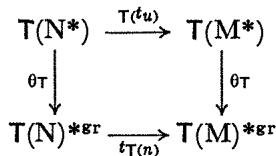
\includegraphics[keepaspectratio]{images/part004_1f4c9f33.jpg}}

is commutative, as follows immediately from the universal property of the tensor algebra (§ 5, no. 1); there are analogous commutative diagrams for \(\theta_{s}\) and \(\theta_{\wedge}\) .

We shall find the homomorphisms \(\theta_{\mathsf{T}}\) , \(\theta_{\mathsf{S}}\) and \(\theta_{\wedge}\) explicitly. For this we consider more generally a coassociative A-cogebra E with coproduct \(c\) and define by induction on \(n\) , for \(n \geqslant 2\) , the linear mapping \(c_{n}\) of E into \(\mathrm{E}^{\otimes n}\) by \(c_{2} = c\) and

\[
c _ {n} = \left(c _ {n - 1} \otimes 1 _ {\mathrm{E}}\right) \circ c.\tag{24}
\]

On the other hand we denote by \(m_{n}:A^{\otimes n}\to A\) the canonical linear mapping such that \(m_{n}(\xi_{1}\otimes\xi_{2}\otimes\cdots\otimes\xi_{n})=\xi_{1}\xi_{2}\ldots\xi_{n}\) and note that, for \(n\geqslant2\) ,

\[
m _ {n} = m \circ (m _ {n - 1} \otimes 1 _ {\mathbf {A}})\tag{25}
\]

writing \(m = m_2\) . With this notation:

Lemma 1. (i) In the associative algebra \(\mathbf{E}^* = \operatorname{Hom}_{\mathbf{A}}(\mathbf{E}, \mathbf{A})\) , the product of \(n\) elements \(u_1, u_2, \ldots, u_n\) of degree 1 is given by

\[
u _ {1} u _ {2} \dots u _ {n} = m _ {n} \circ (u _ {1} \otimes u _ {2} \otimes \dots \otimes u _ {n}) \circ c _ {n}.\tag{26}
\]

\begin{enumerate}
\def\labelenumi{(\roman{enumi})}
\setcounter{enumi}{1}
\tightlist
\item
  Suppose also that the cogebra E is graded. Then, in the graded associative algebra \(\mathbf{E}^{*\mathrm{gr}} = \operatorname{Homgr}_{\mathbf{A}}(\mathbf{E}, \mathbf{A})\) , the product of \(n\) elements \(u_1, u_2, \ldots, u_n\) of degree 1 is given by
\end{enumerate}

\[
u _ {1} u _ {2} \dots u _ {n} = m _ {n} \circ (u _ {1} \otimes u _ {2} \otimes \dots \otimes u _ {n}) \circ \delta_ {n}\tag{27}
\]

where \(\delta_n: \mathbf{E} \to \mathbf{E}^{\otimes n}\) is the linear mapping which maps each \(x \in \mathbf{E}\) to the component of \(c_n(x)\) of multidegree \((1, 1, \ldots, 1)\) .

Formula (26) is just the definition of the product in \(\mathbf{E}^*\) for \(n = 2\) ; to prove it by induction on \(n\) , observe that

\[
\begin{array}{l} u _ {1} u _ {2} \dots u _ {n} \\ \qquad = m \circ ((u _ {1} u _ {2} \dots u _ {n - 1}) \otimes u _ {n}) \circ c \\ \qquad = m \circ ((m _ {n - 1} \circ (u _ {1} \otimes u _ {2} \otimes \dots \otimes u _ {n - 1}) \circ c _ {n - 1}) \otimes u _ {n}) \circ c \\ \qquad = m \circ (m _ {n - 1} \otimes \mathrm{l} _ {\mathrm{A}}) \circ (u _ {1} \otimes u _ {2} \otimes \dots \otimes u _ {n - 1} \otimes u _ {n}) \circ (c _ {n - 1} \otimes \mathrm{l} _ {\mathrm{E}}) \circ c \\ \qquad = m _ {n} \circ (u _ {1} \otimes u _ {2} \otimes \dots \otimes u _ {n}) \circ c _ {n} \end{array}
\]

by virtue of (24), (25), II, § 3, no. 3, formula (5) and the relation

\[
u _ {n} = 1 _ {\mathbf {A}} \circ u _ {n} \circ 1 _ {\mathbf {E}}.
\]

When E is graded and the elements \(u_{i} \in E^{*gr}\) homogeneous of degree 1, then by definition for homogeneous elements \(x_{i} \in E\) ,

\[
(u _ {1} \otimes u _ {2} \otimes \dots \otimes u _ {n}) (x _ {1} \otimes x _ {2} \otimes \dots \otimes x _ {n}) = 0
\]

unless all the \(x_{i}\) are of degree 1, whence formula (27).

It follows from formulae (3), (5) and (7) of no. 1 and formula (24) that when E is taken to be one of the three graded cogebras \(\mathsf{T}(\mathbf{M})\) , \(\mathsf{S}(\mathbf{M})\) and \(\bigwedge (\mathbf{M})\) , we obtain respectively by induction on \(n\) (using the fact that the coproduct is a graded homomorphism of degree 0), for \(x_{1}, x_{2}, \ldots, x_{n}\) in M:

\[
\text { when   } \mathrm{E} = \mathrm{T} (\mathrm{M}), \quad \delta_ {n} (x _ {1} x _ {2} \dots x _ {n}) = x _ {1} \otimes x _ {2} \otimes \dots \otimes x _ {n}
\]

\[
\text { when } \mathrm{E} = \mathrm{S(M)}, \quad \delta_ {n} (x _ {1} x _ {2} \dots x _ {n}) = \sum_ {\sigma \in \mathfrak {S} _ {n}} x _ {\sigma (1)} \otimes x _ {\sigma (2)} \otimes \dots \otimes x _ {\sigma (n)}
\]

\[
\text { when } \mathrm{E} = \bigwedge (\mathrm{M}), \quad \delta_ {n} (x _ {1} x _ {2} \dots x _ {n}) = \sum_ {\sigma \in \mathfrak {S} _ {n}} \varepsilon_ {\sigma}. x _ {\sigma (1)} \otimes x _ {\sigma (2)} \otimes \dots \otimes x _ {\sigma (n)}.
\]

It suffices to note, for example when \(\mathbf{E} = \bigwedge (\mathbf{M})\) , that in the expression \(c_{n}(x_{1}x_{2}\ldots x_{n}) = (c_{n - 1}\otimes 1_{\mathbb{E}})\left(\sum (-1)^{\nu}(x_{i_1}\ldots x_{i_p})\otimes (x_{j_1}\ldots x_{j_{n - p}})\right)\) arising from formula (8) of no. 1, the only terms which can give a term of multidegree \((1,1,\dots ,1)\) are those for which \(n - p = 1\) and hence

\[
\delta_ {n} (x _ {1} x _ {2} \dots x _ {n})
\]

is the term of multidegree \((1, 1, \ldots, 1)\) in the sum

\[
\sum_ {i = 1} ^ {n} (- 1) ^ {n - i} c _ {n - 1} \left(x _ {1} \dots x _ {i - 1} x _ {i + 1} \dots x _ {n}\right) \otimes x _ {i}
\]

and this term is necessarily equal to

\[
\sum_ {i = 1} ^ {n} (- 1) ^ {n - i} \delta_ {n - 1} (x _ {1} \dots x _ {i - 1} x _ {i + 1} \dots x _ {n}) \otimes x _ {i},
\]

whence the result by the induction hypothesis.

Using Lemma 1, the product in \(\mathsf{T}(\mathbf{M})^{*\mathrm{gr}}\) of \(n\) linear forms \(x_{1}^{*}, x_{2}^{*}, \ldots, x_{n}^{*}\) of \(\mathbf{M}^{*}\) is given by

\[
\left\langle x _ {1} ^ {*} x _ {2} ^ {*} \dots x _ {n} ^ {*}, x _ {1} x _ {2} \dots x _ {n} \right\rangle = \prod_ {i = 1} ^ {n} \left\langle x _ {i} ^ {*}, x _ {i} \right\rangle\tag{28}
\]

for \(x_{i} \in \mathbf{M} (1 \leqslant i \leqslant n)\) ; the product of these \(n\) forms in \(S(M)^{*gr}\) is given by

\[
\left\langle x _ {1} ^ {*} x _ {2} ^ {*} \dots x _ {n} ^ {*}, x _ {1} x _ {2} \dots x _ {n} \right\rangle = \sum_ {\sigma \in \mathfrak {S} _ {n}} \left(\prod_ {i = 1} ^ {n} \left\langle x _ {\sigma (i)} ^ {*}, x _ {i} \right\rangle\right);\tag{29}
\]

finally, the product of these forms in \(\bigwedge (\mathbf{M})^{*\mathrm{gr}}\) is given by

\[
\langle x _ {1} ^ {*} x _ {2} ^ {*} \dots x _ {n} ^ {*}, x _ {1} x _ {2} \dots x _ {n} \rangle = \det (\langle x _ {i} ^ {*}, x _ {j} \rangle).\tag{30}
\]

In each of the three cases, we have respectively

\[
\theta_ {T} (x _ {1} ^ {*} \otimes x _ {2} ^ {*} \otimes \dots \otimes x _ {n} ^ {*}) = x _ {1} ^ {*} x _ {2} ^ {*} \dots x _ {n} ^ {*}
\]

\[
\theta_ {S} (x _ {1} ^ {*} x _ {2} ^ {*} \dots x _ {n} ^ {*}) = x _ {1} ^ {*} x _ {2} ^ {*} \dots x _ {n} ^ {*}
\]

\[
\theta_ {\wedge} (x _ {1} ^ {*} \wedge x _ {2} ^ {*} \wedge \dots \wedge x _ {n} ^ {*}) = x _ {n} ^ {*} x _ {n - 1} ^ {*} \dots x _ {1} ^ {*} = (- 1) ^ {n (n - 1) / 2} x _ {1} ^ {*} x _ {2} ^ {*} \dots x _ {n} ^ {*}
\]

and hence we deduce from (28), (29) and (30) the relations

\[
\langle \theta_ {T} (x _ {1} ^ {*} \otimes x _ {2} ^ {*} \otimes \dots \otimes x _ {n} ^ {*}), x _ {1} \otimes x _ {2} \otimes \dots \otimes x _ {n} \rangle = \prod_ {i = 1} ^ {n} \langle x _ {i} ^ {*}, x _ {i} \rangle\tag{28 bis}
\]

(in other words \(\theta_{\mathsf{T}}\) restricted to \(\mathsf{T}^2 (\mathbf{M}^*)\) is just the canonical homomorphism of II, § 4, no. 4)

\[
\langle \theta_ {\mathsf {S}} (x _ {1} ^ {*} x _ {2} ^ {*} \dots x _ {n} ^ {*}), x _ {1} x _ {2} \dots x _ {n} \rangle = \sum_ {\sigma \in \mathfrak {S} _ {n}} \left(\prod_ {i = 1} ^ {n} \langle x _ {\sigma (i)} ^ {*}, x _ {i} \rangle\right)\tag{29 bis}
\]

\[
\begin{array}{r l} (30 \text { bis}) &\langle \theta_ {\wedge} (x _ {1} ^ {*} \wedge x _ {2} ^ {*} \wedge \dots \wedge x _ {n} ^ {*}), x _ {1} \wedge x _ {2} \wedge \dots \wedge x _ {n} \rangle \\ & \qquad = (- 1) ^ {n (n - 1) / 2} \mathrm{det} (\langle x _ {i} ^ {*}, x _ {j} \rangle). \end{array}
\]

PROPOSITION 7. Let \(\mathbf{M}\) be a finitely generated projective A-module. Then the canonical homomorphisms \(\theta_{\mathsf{T}}: \mathsf{T}(\mathbf{M}^{*}) \to \mathsf{T}(\mathbf{M})^{*\mathrm{gr}}\) and \(\theta_{\wedge}: \bigwedge (\mathbf{M}^{*}) \to (\bigwedge (\mathbf{M})^{*\mathrm{gr}})^{0}\) are bijective. Also the graded dual \(\bigwedge (\mathbf{M})^{*\mathrm{gr}}\) is then equal to the dual \(\bigwedge (\mathbf{M})^{*}\) of the A-module \(\bigwedge (\mathbf{M})\) .

Suppose first that \(\mathbf{M}\) has a finite basis \((e_i)_{1\leq i\leq m}\) and let \((e_i^*)_{1\leq i\leq m}\) be the dual basis of \(\mathbf{M}^*\) (II, § 10, no. 4). Formula (28 bis) shows that, for every finite sequence \(s = (j_k)_{1\leq k\leq n}\) of \(n\) elements of the interval \([1,m]\) of \(\mathbf{N}\) ,

\[
\theta_ {\mathsf {T}} (e _ {j _ {1}} ^ {*} \otimes \dots \otimes e _ {j _ {n}} ^ {*})
\]

is the element of index \(s\) in the basis of \((\mathsf{T}^n (\mathbf{M}))^*\) , dual to the basis of \(\mathsf{T}^n (\mathbf{M})\) consisting of the \(e_s = e_{j_1}\otimes \dots \otimes e_{j_n}\) (§ 5, no. 5, Theorem 1). Hence \(\theta_{\mathsf{T}}\) is bijective.

Similarly, formula (30 bis) shows that, for every finite subset \(\mathbf{H}\) of \([1, m]\) with \(n\) elements, \((-1)^{n(n-1)/2} \theta_{\wedge}(e_{\mathrm{H}}^{*})\) (notation of §7, no. 8, Theorem 1) is the element of index \(\mathbf{H}\) in the basis of \((\bigwedge^{n}(\mathbf{M}))^{*}\) , dual to the basis of \(\bigwedge^{n}(\mathbf{M})\) consisting of the \(e_{\mathrm{H}}\) . Hence \(\theta_{\wedge}\) is bijective.

Suppose now only that M is finitely generated and projective; then M is a direct factor of a finitely generated free A-module L, so that there exist two

A-linear mappings \(M \xrightarrow{j} L \xrightarrow{p} M\) whose composition is the identity \(1_{M}\) . We deduce a commutative diagram

\pandocbounded{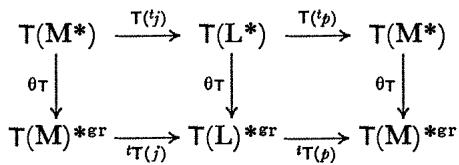
\includegraphics[keepaspectratio]{images/part004_2d3cbe02.jpg}}

and an analogous commutative diagram where \(\mathsf{T}\) is replaced by \(\bigwedge\) . The proposition then follows from the following lemma:

Lemma 2. Let

\pandocbounded{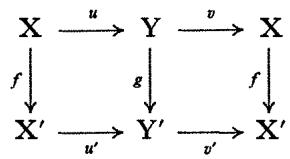
\includegraphics[keepaspectratio]{images/part004_a09507a7.jpg}}

be a commutative diagram of sets and mappings such that \(v \circ u\) and \(v' \circ u'\) are the identity mappings of \(X\) and \(X'\) respectively. Then, if \(g\) is injective (resp. surjective, resp. bijective), so is \(f\) .

u is injective since \(v \circ u\) is, hence, if g is injective, \(u' \circ f = g \circ u\) is injective and therefore f is injective. Similarly \(v'\) is surjective since \(v' \circ u'\) is; hence, if g is surjective, \(f \circ v = v' \circ g\) is surjective and therefore f is surjective.

The last assertion of Proposition 7 follows from the fact that \(\bigwedge (\mathbf{M})\) is then a finitely generated A-module (§ 7, no. 3, Proposition 6 and II, § 11, no. 6, Remark).

We now examine what can be said concerning the homomorphism \(\theta_{\mathsf{S}}\) when \(\mathbf{M}\) is projective and finitely generated. Suppose first that \(\mathbf{M}\) admits a finite basis \((e_i)_{1\leq i\leq m}\) . In the notation at the beginning of the chapter the A-module \(\mathbf{S}^n (\mathbf{M})\) admits as basis the family of elements \(e^{\alpha}\) such that \(|\alpha | = n\) . Let \(u_{\alpha}\) (for \(|\alpha | = n\) ) denote the element of index \(\alpha\) in the basis of \((\mathbf{S}^n (\mathbf{M}))^*\) dual to \((e^{\alpha})\) . The elements \(u_{\alpha}\) , for \(\alpha \in \mathbf{N}^m\) , therefore form a basis of the algebra \(\mathbf{S}(\mathbf{M})^{*\mathrm{gr}}\) and we shall obtain the multiplication table of this basis explicitly. We write

\[
u _ {\alpha} u _ {\beta} = \sum_ {\gamma \in \mathbf {N} ^ {m}} a _ {\alpha \beta \gamma} u _ {\gamma} \quad \text { with } a _ {\alpha \beta \gamma} \in \mathrm{A}.
\]

Then by definition

\[
a _ {\alpha \beta \gamma} = \langle u _ {\alpha} u _ {\beta}, e ^ {\gamma} \rangle = m ((u _ {\alpha} \otimes u _ {\beta}) (c (e ^ {\gamma}))),
\]

where \(m: \mathbf{A} \otimes \mathbf{A} \to \mathbf{A}\) defines the multiplication on \(\mathbf{A}\) and \(c\) is the coproduct of \(\mathsf{S}(\mathbf{M})\) . In other words, \(a_{\alpha \beta \gamma}\) is just the coefficient of \(e^{\alpha} \otimes e^{\beta}\) when \(c(e^{\gamma})\) is written in terms of the basis of \(\mathsf{S}(\mathbf{M})\otimes \mathsf{S}(\mathbf{M})\) consisting of the \(e^{\xi}\otimes e^{\eta}\) , where \(\xi\) and \(\eta\) run through \(\mathbf{N}^m\) . But since \(c\) is an algebra homomorphism,

\[
c (e ^ {\gamma}) = \prod_ {i = 1} ^ {m} (c (e _ {i})) ^ {\gamma_ {i}} = \prod_ {i = 1} ^ {m} (e _ {i} \otimes 1 + 1 \otimes e _ {i}) ^ {\gamma_ {i}}
\]

by formula (4) of no. 1; this gives

\[
c (e ^ {\gamma}) = \sum_ {\xi + \eta = \gamma} (\xi , \eta) e ^ {\xi} \otimes e ^ {\eta}\tag{31}
\]

where we write

\[
((\xi , \eta)) = \prod_ {i = 1} ^ {n} \frac {(\xi_ {i} + \eta_ {i}) !}{\xi_ {i} ! \eta_ {i} !} \quad (\text { cf.   } \S 10, \text {   no.   } 4, \text {   formula   (18) }).\tag{32}
\]

Hence we obtain the multiplication table

\[
u _ {\alpha} u _ {\beta} = ((\alpha , \beta)) u _ {\alpha + \beta}.\tag{33}
\]

On the other hand, if \((e_i^*)_{1\leq i\leq m}\) is the basis of \(\mathbf{M}^*\) , dual to \((e_i)\) , it follows from formula (29 bis) that, for all \(\alpha \in \mathbf{N}^m\) ,

\[
\theta_ {S} (e ^ {* \alpha}) = \alpha ! u _ {\alpha}\tag{34}
\]

in the notation of § 6, no. 6. Hence the homomorphism \(\theta_{\mathsf{S}}\) is bijective if and only if the \(\alpha!u_{\alpha}\) form a basis of \(\mathsf{S}(\mathbf{M})^{*\mathrm{gr}}\) , or also if the elements \(\alpha!1\) are invertible.

PROPOSITION 8. Suppose that the ring A is an algebra over the field Q of rational numbers; then, for every finitely generated projective A-module M, the homomorphism

\[
\theta_ {\mathsf {S}}: S (M ^ {*}) \rightarrow S (M) ^ {* \mathrm{gr}}
\]

is bijective.

It amounts to proving this when M is finitely generated and free; we pass from this to the general case using Lemma 2 as in the proof of Proposition 7.

Remark. Let M be an A-module and \(\rho: \mathbf{A} \to \mathbf{B}\) a commutative ring homomorphism. Then there is a commutative diagram of graded B-algebra homomorphisms

\[
\begin{array}{l} \mathsf {T} ((\mathbf {M} ^ {*}) _ {(B)}) \longrightarrow (\mathsf {T} (\mathbf {M}) ^ {* \mathrm{gr}}) _ {(B)} \\ \mathsf {T} (\upsilon_ {\mathbf {M}}) \Biggl \downarrow \qquad \qquad \qquad \qquad \qquad \qquad \qquad \qquad \qquad \Biggl \downarrow \upsilon_ {\mathbf {T} (\mathbf {M})} \\ \mathsf {T} ((\mathbf {M} _ {(B)}) ^ {*}) \xrightarrow [ \theta_ {\mathsf {T}} ]{} \mathsf {T} (\mathbf {M} _ {(B)}) ^ {* \mathrm{gr}} \end{array}
\]

where the first row is a homomorphism composed of the homomorphism \(\theta_{\mathsf{T}}\otimes 1_{\mathsf{B}}\colon \mathsf{T}(\mathbf{M}^{*})\otimes_{\mathbf{A}}\mathbf{B}\to \mathsf{T}(\mathbf{M})^{*\mathrm{gr}}\) and the canonical isomorphism

\[
\mathsf {T} ((\mathbf {M} ^ {*}) _ {(\mathbf {B})}) \rightarrow \mathsf {T} (\mathbf {M} ^ {*}) \otimes_ {\mathbf {A}} \mathbf {B}
\]

(§ 5, no. 3, Proposition 5). It is immediately verified, using formula (28) and the definition of the homomorphism \(\upsilon_{\mathbf{E}}\) (II, § 5, no. 4), that this diagram is commutative. When \(\mathbf{M}\) is a finitely generated projective A-module, \(\mathbf{M}_{(\mathbf{B})}\) is a finitely generated projective B-module (II, § 5, no. 1, Corollary to Proposition 4) and all the homomorphisms of the above diagram are bijective (Proposition 7 and II, § 5, no. 4, Proposition 8). There are analogous commutative diagrams with \(\mathsf{T}\) replaced by \(\mathsf{S}\) or \(\bigwedge\) ; the diagram for \(\bigwedge\) also consists of bijective homomorphisms when \(\mathbf{M}\) is projective and finitely generated (Proposition 7); if further \(\mathbf{A}\) is an algebra over \(\mathbf{Q}\) , the diagram for \(\mathsf{S}\) also consists of bijective homomorphisms (Proposition 8).

\subsection{INNER PRODUCTS: CASE OF ALGEBRAS}

Let \(E = \bigoplus_{p \geqslant 0} E_p\) be a graded A-algebra of type N and P a graded A-module of type Z; for every homogeneous element \(x \in E_p\) , left multiplication by \(x\) is an A-linear mapping \(e(x)\) of E into itself which is graded of degree \(p\) . For every element \(u \in \text{Homgr}_A(E, P)\) , the right inner product of \(u\) by \(x\) , denoted by \(u \llcorner x\) , is the element \(u \circ e(x)\) of \(\text{Homgr}_A(E, P)\) . We also write \((i(x))(u) = u \llcorner x\) and we see that \(i(x)\) is a graded endomorphism of degree \(p\) of the graded A-module \(\text{Homgr}_A(E, P)\) . If now \(x = \sum_{p \geqslant 0} x_p\) is an arbitrary element of E (with \(x_p \in E_p\) for all \(p \geqslant 0\) , \(x_p = 0\) except for a finite number of values of \(p\) ), we write \(i(x) = \sum_{p=0}^{\infty} i(x_p)\) , which is therefore an endomorphism of the A-module \(\text{Homgr}_A(E, P)\) .

To remember which element, in the expression \(u \llcorner x\) , ``operates'' on the other, observe that the element x which ``operates'' on u is placed at the free end of the horizontal line in \(\llcorner\).

The associativity of the algebra E goes over to the relation \(e(xy) = e(x) \circ e(y)\) for x, y homogeneous; whence, by definition of \(i(x)\) ,

\[
i (x y) = i (y) \circ i (x)\tag{35}
\]

first for \(x, y\) homogeneous and then, by linearity, for arbitrary \(x, y\) in E; this may also be written

\[
(u \llcorner x) \llcorner y = u \llcorner (x y)\tag{36}
\]

for \(x, y\) in \(\mathbf{E}\) and \(u \in \operatorname{Homgr}_{\mathbf{A}}(\mathbf{E}, \mathbf{P})\) ; as on the other hand clearly \(i(1)\) is the identity mapping (since this follows from \(e(1) = 1_{\mathbf{E}}\) ) and \(x \mapsto i(x)\) is A-linear, it is seen that the external law of composition \((x, u) \mapsto u \llcorner x\) ( \(x \in \mathbf{E}\) , \(u \in \operatorname{Homgr}_{\mathbf{A}}(\mathbf{E}, \mathbf{P})\) ) defines, with addition, a right E-module structure on \(\operatorname{Homgr}_{\mathbf{A}}(\mathbf{E}, \mathbf{P})\) .

In particular we consider the case P = A, \(\operatorname{Homgr}_{\mathbf{A}}(\mathbf{E}, \mathbf{P})\) being in this case the graded dual \(E^{*gr}\) of E; \(i(x)\) is then the graded transpose of the A-linear mapping \(e(x)\) (II, §11, no. 6), in other words, for all x, y in E, \(u \in E^{*gr}\) ,

\[
\langle u \llcorner x, y \rangle = \langle u, x y \rangle .\tag{37}
\]

With the convention at the beginning of the paragraph, note that, if \(x \in E_{p}\) , \(i(x)\) is an endomorphism of \(E^{*gr}\) of degree -p.

For every homogeneous element \(x \in \mathbf{E}_p\) , right multiplication by \(x\) is similarly denoted by \(e'(x)\) and the element \(u \circ e'(x)\) of \(\operatorname{Homgr}_{\mathbf{A}}(\mathbf{E}, \mathbf{P})\) , called the left inner product of \(u\) by \(x\) , by \(x \lrcorner u\) ; we write \(i'(x) = x \lrcorner u\) and \(i'(x)\) is therefore a graded endomorphism of \(\operatorname{Homgr}_{\mathbf{A}}(\mathbf{E}, \mathbf{P})\) of degree \(p\) ; as above this definition can be extended to the case where \(x\) is an arbitrary element of \(\mathbf{E}\) . As in this case \(e'(xy) = e'(y)e'(x)\) ,

\[
i ^ {\prime} (x y) = i ^ {\prime} (x) \circ i ^ {\prime} (y)\tag{38}
\]

which may also be written

\[
x \lrcorner (y \lrcorner u) = (x y) \lrcorner u\tag{39}
\]

and shows that the external law of composition \((x,u)\mapsto x\lrcorner u\) defines, with addition, a left E-module structure on \(\operatorname{Homgr}_{\mathbf{A}}(\operatorname{E},\operatorname{P})\) . The associativity of E implies on the other hand that \(e(x)\circ e'(y)=e'(y)\circ e(x)\) for x,y homogeneous in E, whence the relation

\[
(y \lrcorner u) \llcorner x = y \lrcorner (u \llcorner x)\tag{40}
\]

so that the two external laws of composition on \(\mathrm{Homgr}_{\mathbf{A}}(\mathbf{E},\mathbf{P})\) define on this set an (E, E)-bimodule structure (II, § 1, no. 14).

When we take \(\mathbf{P} = \mathbf{A}\) , \(i'(x)\) is the graded transpose of \(e'(x)\) ; in other words, for all \(x, y\) in \(\mathbf{E}\) , \(u \in \mathbf{E}^{*\mathrm{gr}}\) ,

\[
\langle y, x \lrcorner u \rangle = \langle y x, u \rangle .\tag{41}
\]

When the graded algebra E is commutative, obviously \(u \llcorner x = x \lrcorner u\) . When E is anticommutative and P = A, then for \(x \in E_{p}\) , \(y \in E_{r}\) and \(u \in E_{q}^{*}\) , \(yx = (-1)^{pr}xy\) , whence, by (37) and (41), \(\langle u \llcorner x, y \rangle = (-1)^{pr}\langle y, x \lrcorner u \rangle\) . But as the two sides of this relation are zero except for r = q - p,

\[
x \lrcorner u = (- 1) ^ {p (q - p)} u \llcorner x.
\]

Let F be another graded A-algebra and \(\phi: E \to F\) an A-homomorphism of graded algebras; then \(\tilde{\phi} = \operatorname{Hom}(\phi, 1_{P}): \operatorname{Homgr}_{A}(F, P) \to \operatorname{Homgr}_{A}(E, P)\) is a graded A-homomorphism of degree 0; by definition, for \(x, y\) in E and \(u \in \operatorname{Homgr}_{A}(F, P)\)

\[
\begin{array}{r l} (\tilde {\phi} (u \llcorner \phi (x))) (y) & = (u \llcorner \phi (x)) (\phi (y)) \\ & = u (\phi (x) \phi (y)) = u (\phi (x y)) = (\tilde {\phi} (u)) (x y) = (\tilde {\phi} (u) \llcorner x) (y) \end{array}
\]

or also

\[
\tilde {\phi} (u \llcorner \phi (x)) = \tilde {\phi} (u) \llcorner x\tag{42}
\]

and similarly

\[
\tilde {\phi} (\phi (x) \lrcorner u) = x \lrcorner \tilde {\phi} (u).\tag{43}
\]

In other words, when \(\operatorname{Homgr}_{\mathbf{A}}(\mathbf{F}, \mathbf{P})\) is considered as an (E, E)-bimodule by means of the ring homomorphism \(\phi: \mathbf{E} \to \mathbf{F}\) , it is seen that \(\tilde{\phi}\) is an (E, E)-bimodule homomorphism (or also an E-homomorphism of the (F, F)-bimodule \(\operatorname{Homgr}_{\mathbf{A}}(\mathbf{F}, \mathbf{P})\) into the (E, E)-bimodule \(\operatorname{Homgr}_{\mathbf{A}}(\mathbf{E}, \mathbf{P})\) ).

Examples. In particular the above may be applied when E is one of the graded algebras \(\mathsf{T}(\mathbf{M})\) , \(\mathsf{S}(\mathbf{M})\) or \(\bigwedge(\mathbf{M})\) for an A-module M and P an A-module (with the trivial graduation). To find explicitly the bimodule structures thus obtained, note that the elements of degree -n of \(\operatorname{Homgr}_{\mathbf{A}}(\mathsf{T}(\mathbf{M}),\mathbf{P})\) (resp. \(\operatorname{Homgr}_{\mathbf{A}}(\mathsf{S}(\mathbf{M}),\mathbf{P})\) , resp. \(\operatorname{Homgr}_{\mathbf{A}}(\bigwedge(\mathbf{M}),\mathbf{P})\) ) are identified with the n-linear mappings (resp. symmetric n-linear mappings, resp. alternating n-linear mappings) of \(M^{n}\) into P. It suffices to express the products

\[
f \llcorner (x _ {1} \otimes x _ {2} \otimes \dots \otimes x _ {p})
\]

\((\text{resp. } f \llcorner (x_1 x_2 \ldots x_p), \text{ resp. } f \llcorner (x_1 \wedge x_2 \wedge \dots \wedge x_p))\) for every finite sequence \((x_i)_{1 \leq i \leq p}\) of elements of M and the analogues for the left inner product. It follows immediately from the definitions that

\[
f \llcorner (x _ {1} \otimes x _ {2} \otimes \dots \otimes x _ {p}) = (x _ {1} \otimes x _ {2} \otimes \dots \otimes x _ {p}) \lrcorner f = 0\tag{44}
\]

if \(p > n\) and that, for \(p \leqslant n, f \llcorner (x_1 \otimes x_2 \otimes \dots \otimes x_p)\) (resp.

\[
\left(x _ {1} \otimes x _ {2} \otimes \dots \otimes x _ {p}\right) \lrcorner f)
\]

is the \((n - p)\) -linear mapping defined by

\[
\left\{ \begin{array}{l} (f \llcorner (x _ {1} \otimes x _ {2} \otimes \dots \otimes x _ {p})) (y _ {1}, \ldots , y _ {n - p}) \\ = f (x _ {1}, \ldots , x _ {p}, y _ {1}, \ldots , y _ {n - p}) \\ ((x _ {1} \otimes x _ {2} \otimes \dots \otimes x _ {p}) \lrcorner f) (y _ {1}, \ldots , y _ {n - p}) \\ = f (y _ {1}, \ldots , y _ {n - p}, x _ {1}, \ldots , x _ {p}). \end{array} \right.\tag{45}
\]

For \(p > n\) , there are also in \(\operatorname{Homgr}_{\mathbf{A}}(\mathsf{S}(\mathbf{M}), \mathbf{P})\) (resp. \(\operatorname{Homgr}_{\mathbf{A}}(\bigwedge(\mathbf{M}), \mathbf{P})\) ) formulae (44) with \(x_1 \otimes x_2 \otimes \cdots \otimes x_p\) replaced by \(x_1x_2 \ldots x_p\) (resp. \(x_1 \wedge x_2 \wedge \cdots \wedge x_p\) ). For \(p \leqslant n\) , the same substitutions in (45) define the symmetric \((n - p)\) -linear mappings \(f \llcorner (x_1x_2 \ldots x_p)\) and \((x_1x_2 \ldots x_p) \lrcorner f\) (resp. the alternating \((n - p)\) -linear mappings

\[
f \llcorner (x _ {1} \wedge x _ {2} \wedge \dots \wedge x _ {p}) \quad \text { and } \quad (x _ {1} \wedge x _ {2} \wedge \dots \wedge x _ {p}) \lrcorner f).
\]

When \(n = p\) , the above products are equal to the constant function on \(\mathbf{M}\) equal to \(f(x_{1},\ldots ,x_{p})\) .

If \(u: \mathbf{M} \to \mathbf{N}\) is an A-module homomorphism, \(\mathsf{T}(u): \mathsf{T}(\mathbf{M}) \to \mathsf{T}(\mathbf{N})\) is a graded A-algebra homomorphism, then it follows from what we have seen above that \((\mathsf{T}(u))^{\sim}\) is a \(\mathsf{T}(\mathbf{M})\) -homomorphism of the \((\mathsf{T}(\mathbf{N}), \mathsf{T}(\mathbf{N}))\) -bimodule \(\operatorname{Homgr}_{\mathbf{A}}(\mathsf{T}(\mathbf{N}), \mathbf{P})\) into the \((\mathsf{T}(\mathbf{M}), \mathsf{T}(\mathbf{M}))\) -bimodule \(\operatorname{Homgr}_{\mathbf{A}}(\mathsf{T}(\mathbf{M}), \mathbf{P})\) , relative to the ring homomorphism \(\mathsf{T}(u)\) . There are analogous results for \((\mathbf{S}(u))^{\sim}\) and \((\bigwedge(u))^{\sim}\) .
